%\documentclass[8pt,a4paper]{article}
%\usepackage{clrscode}
%\usepackage{url}
%\usepackage[conEntregas]{tp2}
%\usepackage[spanish]{babel} % para que comandos como \today den el resultado en castellano
%\usepackage{a4wide} % márgenes un poco más anchos que lo usual
%\usepackage[T1]{fontenc}
%\usepackage{textcomp}
%\usepackage{graphicx}
%\usepackage{enumitem}
%\newcommand{\subscript}[2]{$#1 _ #2$}
%\usepackage[utf8]{inputenc} 
%\usepackage{pdfpages}
%\usepackage{amsmath}
%\usepackage{vmargin}
%\setpapersize{A4}
%
%%
%\usepackage[utf8]{inputenc}
%\usepackage{fancyvrb}
%\usepackage{xcolor}
%\usepackage{enumitem}
%\usepackage{amssymb}
%\usepackage[conEntregas]{caratula}
%\usepackage{afterpage}
%\usepackage{hyperref}
%\usepackage{wrapfig}
%\usepackage[utf8]{inputenc}
%\usepackage{lmodern}
%\usepackage[T1]{fontenc}
%\usepackage{amsmath}
%\usepackage{graphicx}
%\usepackage{verbatim}
%\usepackage{comment}
%\usepackage{subcaption} 
%\def\infinity{\rotatebox{90}{8}}
%\setlength{\parindent}{12pt}
%\newenvironment{metaverbatim}{\verbatim}{\endverbatim}

\documentclass[11pt,a4paper]{article}
\usepackage{clrscode3e}
\usepackage{url}
\usepackage[conEntregas]{tp2}
\usepackage[spanish]{babel} % para que comandos como \today den el resultado en castellano
\usepackage{a4wide} % márgenes un poco más anchos que lo usual
\usepackage[T1]{fontenc}
\usepackage{textcomp}
\usepackage{graphicx}
\usepackage{enumitem}
\newcommand{\subscript}[2]{$#1 _ #2$}
\usepackage[utf8]{inputenc}
\usepackage{pdfpages}
\usepackage{amsmath}
\usepackage{vmargin}
\setpapersize{A4}
\usepackage{fancyvrb}
\usepackage{xcolor}
\usepackage{amssymb}
\usepackage{afterpage}
\usepackage{hyperref}
\usepackage{wrapfig}
\usepackage[utf8]{inputenc}
\usepackage{lmodern}
\usepackage{verbatim}
\usepackage{comment}
\usepackage{subcaption} 
%\usepackage{algorithm}
%\usepackage{algpseudocode}
\def\infinity{\rotatebox{90}{8}}
\setlength{\parindent}{12pt}
\newenvironment{metaverbatim}{\verbatim}{\endverbatim}
\newenvironment{code}{\fontfamily{cr}\selectfont}{\par}

\usepackage{listings}
\lstset{basicstyle=\fontsize{8}{6}\selectfont\ttfamily,
    breaklines=true,
    numbers=left,
    showstringspaces=false,
	literate=
  {á}{{\'a}}1 {é}{{\'e}}1 {í}{{\'i}}1 {ó}{{\'o}}1 {ú}{{\'u}}1
  {Á}{{\'A}}1 {É}{{\'E}}1 {Í}{{\'I}}1 {Ó}{{\'O}}1 {Ú}{{\'U}}1
  {à}{{\`a}}1 {è}{{\`e}}1 {ì}{{\`i}}1 {ò}{{\`o}}1 {ù}{{\`u}}1
  {À}{{\`A}}1 {È}{{\'E}}1 {Ì}{{\`I}}1 {Ò}{{\`O}}1 {Ù}{{\`U}}1
  {ä}{{\"a}}1 {ë}{{\"e}}1 {ï}{{\"i}}1 {ö}{{\"o}}1 {ü}{{\"u}}1
  {Ä}{{\"A}}1 {Ë}{{\"E}}1 {Ï}{{\"I}}1 {Ö}{{\"O}}1 {Ü}{{\"U}}1
  {â}{{\^a}}1 {ê}{{\^e}}1 {î}{{\^i}}1 {ô}{{\^o}}1 {û}{{\^u}}1
  {Â}{{\^A}}1 {Ê}{{\^E}}1 {Î}{{\^I}}1 {Ô}{{\^O}}1 {Û}{{\^U}}1
  {œ}{{\oe}}1 {Œ}{{\OE}}1 {æ}{{\ae}}1 {Æ}{{\AE}}1 {ß}{{\ss}}1
  {ű}{{\H{u}}}1 {Ű}{{\H{U}}}1 {ő}{{\H{o}}}1 {Ő}{{\H{O}}}1
  {ç}{{\c c}}1 {Ç}{{\c C}}1 {ø}{{\o}}1 {å}{{\r a}}1 {Å}{{\r A}}1
  {€}{{\euro}}1 {£}{{\pounds}}1 {«}{{\guillemotleft}}1
  {»}{{\guillemotright}}1 {ñ}{{\~n}}1 {Ñ}{{\~N}}1 {¿}{{?`}}1
}

\begin{document}
\titulo{Trabajo Práctico 2}
\subtitulo{Clustering}

\fecha{\today}

\materia{Algoritmos y Estructura de Datos III}

\integrante{Buceta, Diego}{001/17}{diegobuceta35@gmail.com}
\integrante{Jim\'enez, Gabriel}{407/17}{gabrielnezzg@gmail.com}
\integrante{Springhart, Gonzalo}{308/17}{glspringhart@gmail.com}

% Pongan cuantos integrantes quieran

\maketitle

\newpage
%\includepdf[pages={1,2}]{tp1.pdf}

\section{Introducción al problema}
%Versear un toque más acá...
En este informe informe vamos a ver distintos problemas cuyas posibles soluciones involucran árboles generadores mínimos y algoritmos que los generan. En particular los problemas son el \textbf{Clustering} y el \textbf{Arbitraje}.

\section{Clustering}
En el mundo del machine learning, problema de \textbf{Clustering} consiste en poder \textbf{agrupar datos} en distintos grupos llamados clusters, donde se espera que los datos de un cluster tengan algún tipo de \textbf{relación o característica} que los \textbf{distinga} de los datos en otros clusters. Este problema es de gran interés ya que tiene muchos usos como por ejemplo:
\begin{itemize}
	\item Las tomografías por emisión de positrones utilizan análisis de clusters para poder diferenciar tejidos en imagenes tridimensionales.
	\item La investigación de mercados utilizan el clustering para poder particionar la población de consumidores en grupos para poder entender mejor la relación entre ellos.
	\item El clustering puede ser utilizado por motores de búsqueda de páginas web para poder agrupar resultados similares.
	\item La segmentación de imágenes utiliza clustering para poder detectar bordes u objetos en imágenes.
\end{itemize}
El análisis de Clusters es un problema de \textbf{aprendizaje no supervisado}, que puede ser abarcado de \textbf{varias maneras}, dependiendo de como uno \textbf{interprete que es lo que constituye un cluster} y como se puede encontrar de forma eficiente. Los diversos algortimos que resuelven el problema se pueden categorizar según su interpretación de lo que es cluster.
Se puede reformular el problema de Clustering como un problema de \textbf{optimización multiobjetivo}, donde el algoritmo y los parámetros (por ejemplo la función para calcular distancias, o la cantidad esperada de clusters) relacionados a este dependen del conjunto de datos a analizar. El análisis de clusters es un \textbf{proceso iterativo} que involucra prueba y error, generalmente es necesario modificar parámetros hasta conseguir los resultados satisfactorios.
% aca estan los usos https://en.wikipedia.org/wiki/Cluster_analysis#Applications
% aca otros https://home.deib.polimi.it/matteucc/Clustering/tutorial_html/
%
%
\subsection{Dificultades del clustering, Aprendizaje Supervisado vs No Supervisado}
%El problema de Clustering es un problema difícil, ya que no existe un algoritmo exacto que pueda generar clusters en tiempo polinomial a partir de un conjunto de datos, además el concepto de un cluster es ambiguo, dado un grafo no existe una única configuración de clusters que separe los datos, sino que hay varias configuraciones que a simple vista pueden parecer válidas.
%El análisis de Clusters es un problema de \textbf{aprendizaje no supervisado}, eso significa que no se sabe nada a priori sobre el conjunto de datos inicial.
Como se mencionó anteriormente el análisis de clusters es un problema de \textbf{aprendizaje no supervisado}, para poder entender como esto afecta al problema vamos a explicar de forma resumida los dos tipos principales de aprendizajes que existen en el mundo del machine learning.

\subsubsection*{Aprendizaje Supervisado}
El Aprendizaje Supervisado es una técnica de machine learning que, a partir de conjuntos de entrenamiento de entradas y salidas esperadas, utiliza un algoritmo que intenta inferir una función que pueda predecir las salidas adecuadas para cualquier entrada nueva. Se llama supervisado ya que a medida que el algoritmo hace predicciones sobre los conjuntos de entrenamiento se van corrigiendo los datos de acuerdo a las salidas esperadas. Los problemas de aprendizaje supervisado se pueden agrupar en problemas de \textbf{clasificación}, cuando las salidas son clases o categorías y problemas de \textbf{regresión}, cuando las salidas son valores reales.

\subsubsection*{Aprendizaje No Supervisado}
A diferencia del aprendizaje supervisado, en el \textbf{aprendizaje no supervisado} no se sabe nada de la información de entrada \textbf{a priori}. A partir de un conjunto de datos de entrada se corren algoritmos que se encargan de descubrir estructuras o características en los datos. Como no hay salidas esperadas, la única forma de saber si los datos resultantes de correr los algoritmos son correctos es realizar evaluaciones sobre los resultados. Pese a esta desventaja, el aprendizaje no supervisado es útil cuando por ejemplo, no se sabe nada sobre los datos a estudiar, por lo que se puede usar un algoritmo de este tipo para obtener información sobre los mismos.

Entonces podemos ver que el problema de análisis de clusters cae en la segunda categoría de aprendizaje, esto lo hace un problema difícil, ya que no existe una solución "correcta" con la que podríamos revisar los resultados obtenidos del los algoritmos de clustering, además por lo mencionado anteriormente, la definición de cluster en si es ambigua y dependiendo de lo que se decida definir como un cluster, los resultados obtenidos sobre un mismo conjunto de datos de entrada pueden ser muy diferentes.

%(Explicación de porque el clustering es hard)

%\subsection{Aprendizaje Supervisado vs No Supervisado}

%PONER LO DE LOS APRENDIZAJES
%https://en.wikipedia.org/wiki/Supervised_learning
%https://en.wikipedia.org/wiki/Unsupervised_learning

%Hay que confirmar esto de acá abajo, creo que se cumple esto pero habría que ver algun paper o página que diga que esto es así. Agrandar un touch el primer párrafo de acá
\subsection{Heuristica para resolver el problema}

Para resolver el problema utilizamos un algoritmo basado en el método de detección de clustes explicado en el paper "Graph-Theoretical Methods for Detecting and Describing Gestalt Clusters" de Charles T. Zahn, y su forma de calcular los clusters es la siguiente: Consideramos nuestros datos como una serie de puntos en un plano, tomando un grafo completo $G$ usando los puntos como vertices y las distancias entre ellos como pesos en las aristas. Luego calculamos el Árbol Generador Mínimo de $G$ y lo llamamos $T$.
Para poder encontrar los clusters hay que eliminar de $T$ a los ejes \textbf{inconsistentes}, según el paper un eje $e$ es inconsistente si su peso supera en cierta cantidad de desviaciones estandard a las medias de los pesos de las aristas que estén a distancia $k$ de los vértices que están en sus puntas. Al remover un eje inconsistente, las componentes conexas formadas son identificadas con un indice, entonces luego de recorrer todas las aristas, todas las componentes conexas van a tener un  indice distinto y podemos interpretarlas como los clusters del grafo.
Para poder calcular el AGM del grafo $G$ se implementaron dos algoritmos, el algoritmo de Kruskal y el algoritmo de Prim, ambos levemente modificados para utilizar estructuras de Lista de Incidencia y Lista de Adyacencia respectivamente. Además, se implentaron dos versiones de Kruskal, una con path-compression y otra sin, a fin de poder compararlos en la experimentación.
%Agregar nota en el parrafo de abajo, aunque puede que lo saquemos later

\subsection{Principios de la Forma (Gestalt Principles)}

%AMPLIAR UN CACHO ESTOOOOOOOOOOO
El método de detección de clusters esta basado en los \textit{principios de la forma de organización perceptible} que están explicados en el paper anteriormente mencionado, en resumen se intento formular un método matemático que detecte clusters utilizando los principios de tal forma que los clusters formados correspondan con los que una persona podría percibir al ver el grafo.
Los diversos principios explican como la percepción humana organiza datos sensoriales visuales, reconoce patrones y simplifica imágenes complejas. El principio fundamental para la detección de clusters es el \textbf{principio de la proximidad} que dice: "Los objetos o formas que se encuentren cerca unos de otros aparentan \textbf{formar grupos}", incluso si los objetos o formas son muy diferentes van a parecer formar parte de un grupo si se encuentran \textbf{cerca}. En este principio, el sentido de que dos objetos estén cerca no necesariamente es el de que su distancia sea corta, varios objetos pueden ser agrupados siguiendo este principio pero aplicado sobre otras características de los mismos, como sus tamaños, sus formas, sus colores, etc.
%Explica como los algos del paper se basan de esto, o otros algos así se le da un cierre al tema

\section{Justificación teórica}

\subsection{Arboles Generadores Mínimos}
%Explicar acá lo del papeeeeeeeeeeeeeeer
En el método explicado anteriormente los clusters se calculan sobre un AGM del grafo completo de los datos, nos interesaría saber como es que el AGM nos garantiza que se van a calcular todos los clusters que pueda haber en el grafo, para eso vamos a ver primero algunos conceptos.
Si tenemos un grafo $G$ podemos pensar que una particion de $G$ es una división en dos subconjuntos no vacíos $(P, Q)$, luego definimos la distancia $p(P, Q)$ entre particiones como el peso más chico entre los ejes que tienen un nodo en $P$ y otro en $Q$. Luego podemos pensar en dos conjuntos de ejes del grafo $C(P, Q)$ es el conjunto de ejes que tienen un nodo en $P$ y el otro nodo en $Q$, de estos ejes llamamos \textbf{cadena} a los ejes cuyo peso sea igual a $p(P, Q)$ y definimos $\lambda(P, Q)$ como el conjunto de cadenas de $P$ y $Q$.
En un grafo con pesos en los ejes resulta útil definir el costo de un camino en el grafo como el \textbf{peso máximo} entre los pesos de los ejes que forman parte del camino, de esta forma podemos definir también a un camino entre dos nodos como \textbf{minimax} si es el camino con menor peso entre ellos.
Ahora con estos conceptos podemos presentar los siguientes teoremas\footnote{Estos teoremas están demostrados en el apéndice (para los teoremas 1-3) y en las referencias (para el teorema 4) del paper de C.T. Zahn, que se encuentra en la bibliografía} :
\begin{itemize}
	\item Teorema 1: Para cada partición $(P, Q)$ de $G$, cualquier AMG contiene al menos un eje de $\lambda(P, Q)$.
	\item Teorema 2: Todos los ejes del AGM son ejes cadena de alguna partición de $G$.
	\item Teorema 3: Si $S$ son los nodos de $G$ y $C$ es un subconjunto no vacío de $S$ tal que para toda partición $(P, Q)$ de $C$ se cumple que $p(P, Q) < p(C, S-C)$ entonces restringir un AGM a los nodos de C forma un subarbol del AGM.
	\item Teorema 4: Si $T$ es un AGM de $G$ y $X$ e $Y$ son nodos de $G$, entonces el camino único en $T$ que va de $X$ a $Y$ es un camino minimax entre $X$ e $Y$.
\end{itemize}

De estos teoremas el más importante es el tercero, del cual se puede concluir que los clusters van a ser subarboles del AGM , de los teoremas 1 y 2 vemos que los ejes que conectan a los clusters son los de menor peso y el teorema 4 nos asegura que el camino entre nodos va a ser minimax y entonces los nodos conectados no van a tender a alejarse del cluster donde pertenecen.

\section{Algoritmos presentados}

\subsection{Aclaraciones}
\begin{itemize}
	\item El tipo peso es un alias del tipo float
	\item El tipo AristaAd consiste de un Nodo llamado \textbf{adyacente} y un \textbf{peso} funciona a como una tupla
	\item El tipo Arista contiene dos nodos, \textbf{desde} y \textbf{hasta}, un \textbf{índice} y un \textbf{peso}, y comparadores de igualdad y orden (Que se realizan en $O(1)$) 
\end{itemize}

%ARREGLAR ESTOS O CAMBIARLOS A UNA VERSION QUE USE OTRO PAQUETE
%2018-10-24 HAY QUE CAMBIAR TODOOOOOOOOOOOOOO SE HACE LO MAS RAPIDO POSIBLE
\subsection{Kruskal}
\begin{codebox}
  	\Procname{$\proc{KruskalSinPathComp}(ListaIncidencia: grafoCompleto, cantNodos: entero)$}
		\li padre $\gets$ vector de enteros de tamaño de cantNodos y cargado con el valor
		\zi 	 de su posición en cada posición
		\li AGM $\gets$ lista de incidencia vacia, de tamaño cantNodos-1
		\li OrdenarPorPeso(grafoCompleto)
		\li \For{e:Arista $\in$ grafoCompleto} \Do
			\li \If $getPadre(indice(e.primerNodo), padre) == getPadre(indice(e.segundoNodo),padre)$ \Then
					\li agregar(e,agm)
				\End
			\End
	\li Devolver AGM
\end{codebox}

\begin{codebox}
\Procname{$\proc{getPadre}(entero: indice, padre: vector de enteros)$}
\li \If $padre[indice] == indice$ \Then
		\li Devolver indice
\li \Else
		\li getPadre(indice(padre[indice]), padre)
\li \End
\end{codebox}


\begin{codebox}
\Procname{$\proc{getPadreConPathComp}(entero: indice, padre: vector de enteros, altura:vector de enteros, nivelesSubidos: entero$}
\li \If $padre[indice] == indice$ \Then
		\li altura[indice] $\gets$ nivelesSubidos
		\li Devolver indice
	\li \Else
		\li padre[indice] $\gets$ getPadreConPathComp(indice(padre[indice]),padre,altura,nivelesSubidos+1)
		\li Devolver padre[indice]
		\End
\end{codebox}

\begin{codebox}
\Procname{$\proc{unirPadres}(indiceNodo1: entero, indiceNodo2:entero, padre: vector de enteros)$}
	\li padreNodo1 $\gets$ getPadre(indiceNodo1, padre)
	\li padre[indiceNodo2] $\gets$ padreNodo1
\end{codebox}

\begin{codebox}
\Procname{$\proc{unirPadresConPathComp}(indiceNodo1: entero, indiceNodo2:entero, padre: vector de enteros, altura:vector de enteros, nivelesSubidos: entero)$}
\li padreNodo1 $\gets$ getPadreConPathComp(indiceNodo1, padre,altura,0)
\li padreNodo2 $\gets$ getPadreConPathComp(indiceNodo2, padre,altura,0)
\li padreMenosAltura $\gets$ min(altura[padreNodo1],altura[padreNodo2])
\li padreMasAltura $\gets$ max(altura[padreNodo1],altura[padreNodo2])
\li padre[padreMenosAltura] $\gets$ padreMasAltura
\end{codebox}

\subsection{Prim}

\begin{codebox}
\Procname{$\proc{PrimConCola}(G: ListaAdyacencias)$}
\li $res \gets$ Crear vector de pesos del tamaño de la lista G con valor $\infty$ en cada pos
\li $padres \gets$ Crear vector de Nodos del tamaño de la lista G
\li $visitados \gets$ Crear vector de booleanos del tamaño de la lista G con valor $False$ en cada pos
\li $cola \gets$ Crear cola de prioridad vacia que tome AristaAd 
\zi y los ordene en orden ascendiente según su peso
\li Encolar el una AristaAd que tenga como adyacente al primer nodo de $G$ y como peso $0$ en $cola$
\li \While{not $cola.vacia()$} \Do
\li 	$u \gets$ $cola.siguiente()$
\li 	$cola.pop()$
\li 	$visitados[u.adyacente.indice] = True$
\li 	\For{$AristaAd$ ad : $G[u.adyacente]$} \Do
\li 		\If{not $visitados[ad.adyacente.indice]$} \Then
			\li $cola.encolar(ad)$
\li 			\If{$res[ad.adyacente.indice] > ad.peso$} \Then
					\li $res[ad.adyacente.indice] \gets ad.peso$
					\li $padres[ad.adyacente.indice] \gets u.adyacente$
				\End
			 \End
		\End
	\End
\li Devolver $padres$
\end{codebox}

\begin{codebox}
\Procname{$\proc{PrimSinCola}(G: ListaAdyacencias)$}
\li \Comment $G$ se pasa por referencia
\li $distancia \gets$ Crear vector de pesos del tamaño de la lista G con valor $\infty$ en cada pos
\li $padres \gets$ Crear vector de Nodos del tamaño de la lista G
\li $visitados \gets$ Crear vector de booleanos del tamaño de la lista G con valor $False$ en cada pos
\li $first \gets G[0]$
\li 
\li \For{$AristaAd$ elem : $G[first]$} \Do 
\li		$distacia[elem.adyacente.indice] \gets elem.peso$
\li 	$padres[elem.adyacente.indice] \gets first$
	\End
\li 
\li $distacia[first.indice] \gets 0$
\li $visitados[first.indice] \gets true$
\li 
\li \While{not $todosVisitados(visitados)$} \Do 
\li 	$v \gets menorNoVisitado(G.getNodos(), distacia, visitados)$
\li 	$visitados[v.indice] \gets true$
\li 	\For{$AristaAd$ elem : $G[v]$} \Do
\li 		\If{not $visitados[elem.adyacente.indice]$} \Then
\li 			\If{$distacia[elem.adyacente.indice] > elem.peso$} \Then
\li 				$distacia[elem.adyacente.indice] \gets elem.peso$
\li 				$padres[elem.adyacente.indice] \gets v$
				\End
			\End
		\End
	\End
 
\li Devolver $padres$
\end{codebox}

Nota: todosVisitados devuelve en tiempo lineal si todos los elementos del vector de booleanos que toma son verdaderos y menorNoVisitado devuelve el nodo con menor distancia que no fue visitado aún, también en tiempo lineal.

\subsection{Clustering}

\begin{codebox}
\Procname{$\proc{armarGrafoCompleto}(nodos:vector de Nodos)$}
\li listaAristas $\gets$ inicializar lista de incidencia
\li matrizAristas $\gets$ inicializar matriz de adyacencia
\li
\li \For $i \gets 0$ \To $tam(nodos)$ \Do
\li 		\For  $j \gets i+1$ \To $tam(nodos)$ \Do
					\li armar arista con datos de v[i] y v[j]
					\li agregar arista a listaAristas
				\End
		\End
\li
\li armar matriz de adyacencia con la lista de incidencia
\li Devolver Matriz de adyacencia y Lista de incidencia
\end{codebox}

\begin{codebox}
\Procname{$\proc{retirarEjesInconsistentes}(ListaIncidencia ls, \sigma_{T}, profVecindario, f_{T}, forma, cantidadDeClusters, padre: vector de enteros )$}
\li $la \gets $ Crear lista de adyacencia a partir de $ls$
\li Marcar el representante de todos los nodos con $0$
\li 
\li \For $Arista$ e : $ls$ \Do
\li 	\If{not $e.indice == -1$} \Then
\li			\If{forma == 1} \Then
\li 			Calcular media y desviación respecto del vecindario de los 
\zi				extremos de $e$, avanzando con profVecindario profundidad
\li 			\If{$e$ es inconsistente} \Then
\li 				Saco a $e$ de $la$ y $ls$
\li 				Recorro en $la$ los nodos alcanzables desde un extremo y marco
\zi					su padre como $cantidadDeClusters$
\li 				$cantidadDeClusters++$
				\End
\li 		\Else
\li				Se realiza el mismo procedimiento que antes pero se utiliza 
\zi 			el segundo criterio de inconsistencia
			\End
		\End
	\End
\end{codebox}

\subsection{Complejidad}
%Acá espero a lo que me diga Diego
Ahora vamos a ver las complejidades de los algortimos presentados, los algoritmos de Kruskal y Prim utilizados son los que se explicaron en clase, y de la forma en la que fueron programados las complejidades no fueron afectadas.
\\
Entonces para KruskalSinPathComp, getPadre es $O(n)$
%Lo DEJO ASI TOO MIENTRAS

Para PrimSinCola, el for al principio es $O(n)$ como cada Nodo agregado se marca y hay $n$ nodos, sabemos que el ciclo while a lo sumo se ejecuta $n$ veces, dentro de cada ciclo se calcula el nodo con distancia mínima en $O(n)$, y se acutalizan las distancias de los nodos adyacentes al mínimo en $O$(cantidad de nodos adyacentes al mínimo) que a lo sumo es $n$, entonces su complejidad también es $O(n^2)$.

%Lo dejo por ahora
En PrimConCola, a partir de un nodo inicial, se van encolando las aristas que vayan a nodos no visitados, a lo sumo la cantidad de aristas es $2m$, obtener el primero de la cola es $O(\log n)$ y en $O()$

\subsubsection{Cálculo de ejes inconsistentes}
Para buscar ejes inconsistentes vamos a aprovechar las ventajas que nos brindan las implementaciones de listas de adyacencia y incidencia. \\
La idea es la siguiente: vamos a recorrer todas las aristas, sacándolas de la lista de incidencia y calcular con un método parecido a BFS los promedios de longitud de vecino, desviaciones, etc. Hay m aristas (que por estar trabajando con un AGM son $\approx$ n) y por cada una calcular esas cosas es $O(n+m)$ $\approx$ $O(n)$. En caso de ser considerado consistente vamos a recorrer, también con algo parecido a BFS, los nodos alcanzables desde uno de los extremos de la arista considerada inconsistente y le vamos a modificar su representante, con un vector de n posiciones donde en la posición i-ésima está el representante del nodo i-ésimo. Por temas de implementación, si la arista es inconsistente vamos a eliminarla de la siguiente forma: en la lista de incidencia modificamos su indice a -1, que es un valor que consideramos internamente como arista no disponible, y en la lista de adyacencia sí la eliminamos, accediendo en tiempo constante a la posicion del vector de ese nodo y con un iterador recorriendo sus nodos vecinos hasta encontrar el que corresponde con el otro extremo de la arista. Esto cuesta O(m) $\approx$ O(n), porque para cada nodo se recorre a lo sumo su grado y si se hace para todos los nodos será la suma de los grados de los nodos que es asintóticamente m, que por ser un árbol es O(n).\\
La complejidad total sería O($n^{2}$). Usar ambas listas nos permite tener los beneficios de recorer y 'deshabilitar' si es necesario las aristas en tiempo constante por la lista de incidencia y utilizar una modificación de BFS para poder calcular lo necesario y reasignar los representantes en caso de ser necesario de forma óptima por la lita de adyacencia.

\subsubsection{Procesamiento de puntos en el espacio}
Una vez leídos y almacenados en un vector todos los puntos del espacio ingresados, se procesarán uno a uno utilizando el siguiente procesamiento: por cada uno de ellos se recorrerán todos los que vengan después (en orden de ingreso). Esto nos asegura que cada nodo estará conectando con todos los demás (excepto él mismo) y así conseguiremos el grafo completo que tiene como nodos a los puntos ingresados. Esto lo conseguimos con complejidad O($n^{2}$). Construimos con esto la lista de incidencia y matriz y lista de adyacencia.\\
Para generar el AGM de kruskal, tenemos funciones que permiten facilitar el entendimiento del pseudocódigo correspondiente. Básicamente se procesa cada arista de la lista de incidencia del grafo completo, previamente ordenadas ( ordenada con el sort de C++ en O($\log{m}$ * m), donde m $\approx$ $n^2$), y se comprueba si la arista tomada actual (que es la de mínimo peso) genera un ciclo en las ya agregadas. Esto se hace mediante una implementación de funciones de UDS (Union Disjoint Set) que nos permite la manipulación de conjuntos de cosas disjuntas como las componentes conexas de un grafo. Una de estas funciones permite encontrar el representante de un punto/nodo (inicialmente cada nodo es su propio representante), lo que sería equivalente a preguntar a que componente conexa corresponde y en caso de ser de diferentes se agrega la arista, si no se sigue a la siguiente. Si la arista se elige se deben actualizar los representantes. Vamos a representar a los nodos en árboles y cada padre será el representante de un nodo, excepto la raíz que será su propio padre. Para mejorar la eficiencia, vamos a almacenar además del padre de cada nodo su altura. Imaginemos que cada representante sería la raíz de un árbol y al momento de buscar el representante de una de los hijos, 'subiríamos' hacia arriba preguntando por el padre de ese nodo, que en caso de no ser la raíz no será su propio representante y nos enviará hacia su padre. Este padre si no es la raíz, tampoco tendrá como representante a él mismo y nos enviará a su representante, así hasta llegar a la raíz. Durante toda esta búsqueda vamos a hacer dos cosas: se actualizará al nodo actual el representante y además se actualizará la altura del nodo que busquemos su representante, aumentando en 1 cada vez que subíamos un nivel en el árbol. Almacenar estas cosas nos sirve para: en primer lugar, la próxima vez que preguntemos por el representante de algún nodo de ese árbol no será necesario realizar otra vez todo ese recorrido (Path compression) porque estarán actualizados los representantes, y por otro lado al momento de unir las componentes conexas, tenemos podemos 'colgar' el árbol más chico del otro, realizando menos operaciones. Además la complejidad de buscar un representante será a lo sumo la altura del árbol (de a lo sumo n nodos) al que pertenece.\\
Así, al momento de unir las componentes conexas, simplemente actualizamos el representante del árbol más chico ( O(encontrar representante(nodo) $\approx$ O(altura árbol(nodo)) con el más grande. Entonces buscar un representante y unir componentes $\in$ O(log n).
\\Siguiendo con la explicación, el procesamiento de todas las aristas ( donde m $\approx$ $n^{2}$)sería O($n^2$ * $\log$ n + $\log$ $n^{2}$ * $n^{2}$) $\approx$ O($\log$ $n^{2}$ * $n^{2}$) $\approx$ O($\log$ $n$ * $n^{2}$).

\section{Experimentación}
\subsection{Variaciones}
\begin{verse}
Tomaremos los casos de test brindados en http://cs.joensuu.fi/sipu/datasets/ y correremos nuestro algoritmo para poder obtener las clusterizaciones.\\
Los experimentos estarán centrados en analizar las diferentes tipos clusterizaciones que pueden realizarse variando las definiciones de eje inconsistente. Intentaremos analizar las configuraciones necesarias para que se pueda alcanzar una clusterización lo más cercana a la de la percepción humana y los resultados interesantes al que pueden llegarse. Para cada clusterización utilizaremos como solución previa los AGM obtenidos por los algoritmos de Kruskal, Kruskal con path compression y Prim, y a su vez indicaremos en cada caso las mediciones de tiempo correspondientes.  Para ello usaremos la porción de código utilizada en clase para medir tiempos con una cantidad de tres repeticiones de cada uno para una mejor precisión.\\

Dados los siguientes: $f_{T}$ multiplicador del promedio, $\sigma_{T}$ multiplicador de la desviación, y la profundidad del vecindario de los extremos del eje candidato, W(XY) el peso del eje candidato, y sea X e Y sus nodos extremos, definiremos un eje inconsistente:
\begin{itemize}
\item Forma 1: $\frac{W(XY)}{Promedio(Vecindario(X))}$ $>$ $f_{T}$ $  y $ $\frac{W(XY)}{Promedio(Vecindario(Y))}$ $>$ $f_{T}$, \\Es decir, la proporción entre el peso del eje candidato y el promedio de peso del vecindario de sus extremos es mayor al coeficiente dado.
\item Forma 2: $W(XY) >  Promedio(Vecindario(X)) + \sigma_{T}$ $ * $ $ desviacion(Vecindario(X)) $ $ y$ $W(XY) >  Promedio(Vecindario(Y)) + \sigma_{T}$ $ * $ $ desviacion(Vecindario(Y)) $, \\Es decir, que el peso del eje candidato supere al promedio del vecindario de sus extremos por al menos $\sigma_{T}$ unidades de la desviación del vecindario del extremo, y además se cumpla la forma 1.
\end{itemize}



Comencemos señalizando que la clusterización no es un problema matemáticamente definido y por ello podemos definirlo de forma tal que se obtenga diferentes resultados para mismas situaciones. 
La clusterización es la organización y detección de patrones en nuestros datos en grupos que tengan algún significado. Por lo general, a partir de un lote de datos, se busca caracterizarlos en base a la información que se pueda obtener de ellos y no por un patrón o clase de datos conocida dada. Es decir, no se separan los datos en función de su característica en propiedades o atributos previamente fijados, sino que se evalúa la correlación de cada uno de ellos entre todos los datos y en función de esto se agrupan. Estos analisis suelen dividirse como analisis supervisado y no supervisados (o clusteing), donde en los supervisados se cuenta inicialmente con las caracterizaciones que se esperan obtener y se analizan los datos para el reconocimiento de los patrones que permitan situarlo en el modelo correcto. Algunos ejemplos son redes neuronales, árboles de decisión, etc. Discutir el significado de correlación y significancia depende en gran medida de la naturaleza de los datos que se organicen. En nuestro caso, tenemos datos númericos correspondientes a puntos en el plano y en donde vamos a tomar como relación primaria entre ellos como su distancia euclídea. Experimentaremos con casos ya conocidos de clusterización y evualuaremos fuertemente la habilidad del modelo y sus parámetros para acercarse a los resultados de nuestra percepción, aunque siempre teniendo en mente la literatura del problema de clusterización y particularmente los analisis de los principios de agrupación propuestos por la filosofía de Gestalt previamente analizados.\\
Además, vamos a referirnos al método utilizado para la generación del AGM para referirnos a una determinada clusterización. Vamos a utilizar los datasets provistos por: \url{http://cs.joensuu.fi/sipu/datasets/}

\subsection{Experimentación}

\begin{verse}
Comenzaremos la parte de experimentación exponiendo algunos casos particulares de lo que se trata la clusterización.
\begin{center}
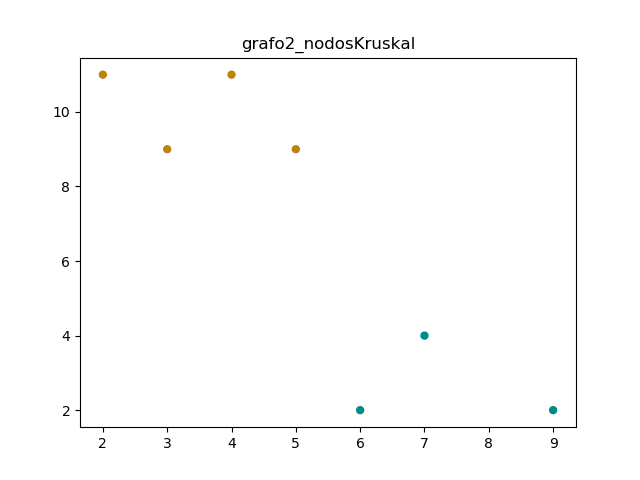
\includegraphics[scale=.8]{graficos/grafo2_nodosKruskal.png}
\end{center}
Intuitivamente los colores marcan ciertas diferencias entre los conjuntos de puntos. A simple vista los  naranja no parecen ser del mismo tipo que los azules, aunque habría que definir que significa eso técnicamente. En este caso estamos suponiendo que dos uniones de puntos que tengan distancia diferente son de diferente tipo. En este caso 'distancia diferente' significa una diferencia del doble de largo. Pero esta claro que en otro contexto dos cosas diferentes necesiten ser 'más' diferentes y la diferencia tenga que ser por ejemplo del triple y entonces acá no habría más que un grupo de puntos. Pero también podría ser lo contrario y considerar que dos puntos separados por una distancia muy chica ya son de diferente tipo y entonces podríamos conseguir que cada punto sea de un tipo diferente. A todo esto podemos involucrar las desviaciones que existen entre vecinos de puntos, porque podríamos querer ser un poco más restrictivos respecto de que separar, puede que en nuestro contexto nos importe cómo están distribuidos los vecinos de un punto más allá de las distancias que los separen. 
\begin{center}
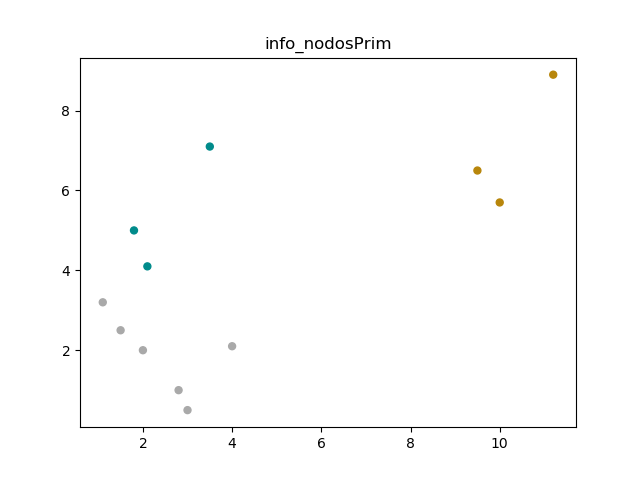
\includegraphics[scale=.8]{graficos/info_nodosPrim.png}
\end{center}
Por ejemplo en este caso, del lado izquierdo tenemos una serie de puntos que no parecen estar lo suficientemente alejados y sin embargo las desviaciones entre sus vecinos nos permiten ser más restrictivos con la medición.
\end{verse}

Con esta breve introducción, planteamos algunos interrogantes que pueden surgir y que sería interesante investigar en un análisis más profundo y completo de una mayor variedad de casos.

\subparagraph{Cómo conseguir clusters parecidos a nuestra percepción? Es siempre posible? Cómo varían los diferentes métodos de búsqueda de AGM para la clusterización? Como afectan a la clusterización la variación de los parámetros definidos para considerar un eje inconsistente?}


\subsection{Dataset: Aggregation}
\begin{center}
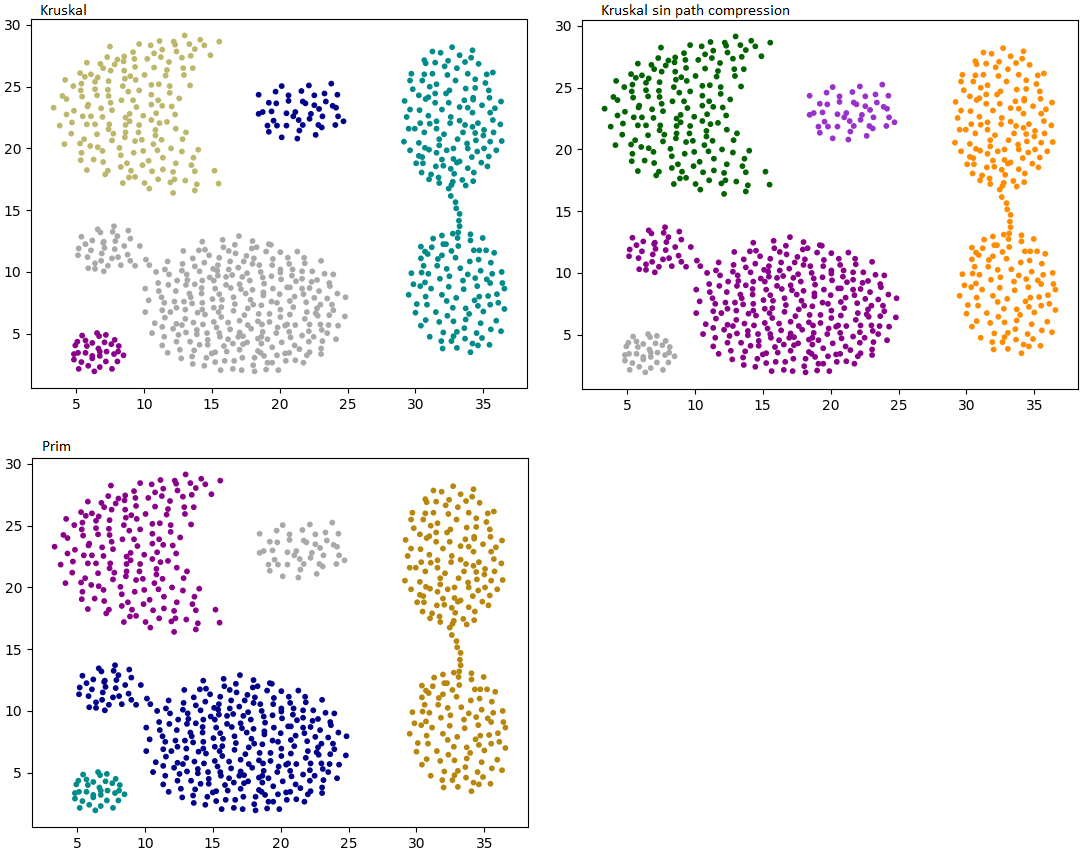
\includegraphics[scale=.5]{graficos/aggregation.png}
\end{center}

\subsubsection{Tiempos}
\begin{table}[ht]
\caption{Tiempos de ejecución en milisegundos} % title of Table
\centering % used for centering table
\begin{tabular}{c c c c} % centered columns (4 columns)
\hline\hline %inserts double horizontal lines
Cant.Puntos & Kruskal & Kruskal sin path comp & Prim \\ [0.5ex] % inserts table
%heading
\hline % inserts single horizontal line
788 & 254.66 & 386.66 & 151.66 \\ [1ex] % [1ex] adds vertical space
\hline %inserts single line
\end{tabular}
\label{table:nonlin} % is used to refer this table in the text
\end{table} 

Analizando el siguiente caso podemos ver que generando el AGM con cualquiera de los métodos elegidos obtenemos la misma clusterización. Elegimos como parámetros que un eje inconsistente debe superar en 2.5 al promedio de los vecinos de 2 pasos de sus extremos. La clasificación resulta en 5 clusters. Como primera observación, la percepción humana podría arrojar que el cluster de la esquina derecha en realidad podrían ser dos clusters diferentes, al igual que el cluster de la esquina izquierda. Si intentamos conseguir algo más cercano a esto, podemos intentar clasificar ahora también teniendo en cuenta la desviación. Como todos los puntos tienen una densidad de vecinos parecida, no tiene mucho sentido modificar la distancia del vecindario de los extremos (actualmente dos). Si reducimos el coeficiente del promedio de 2.5 hasta 1.4 y el coeficiente de la desviación lo fijamos en 2, d = 2. Después de varios intentemos, encontramos que en ese punto obtenemos lo siguiente:


\begin{center}
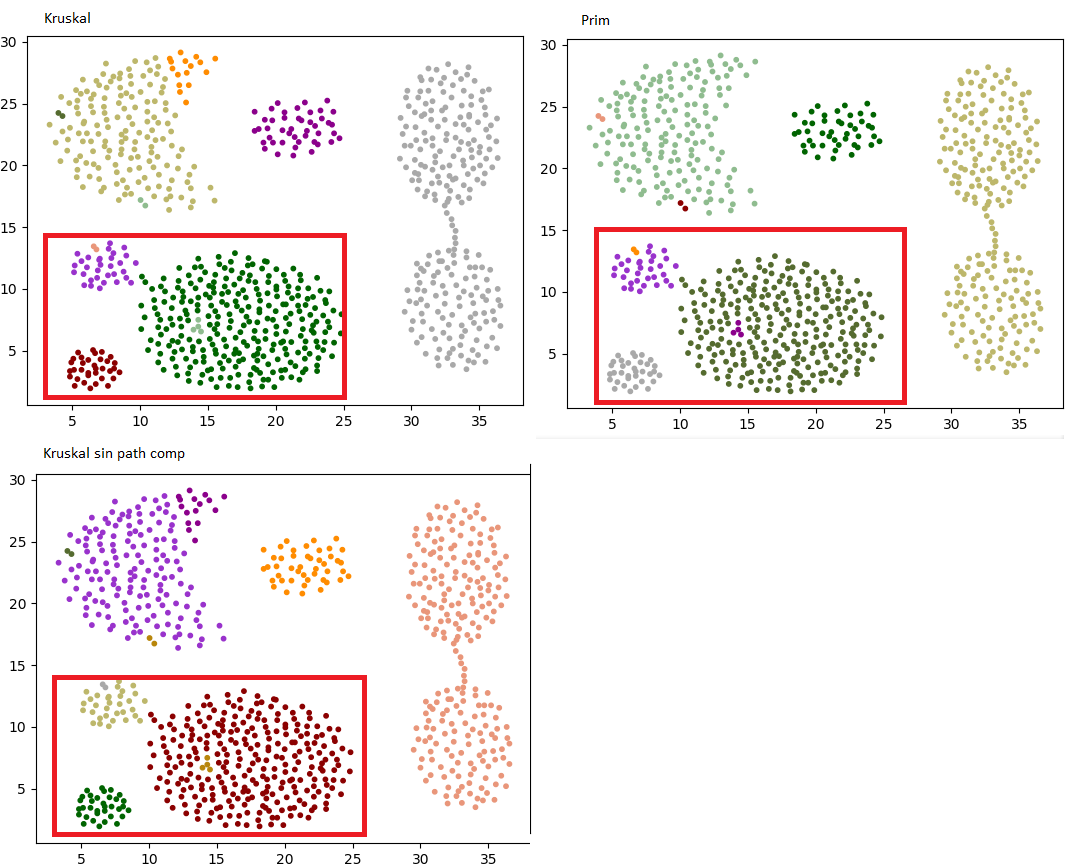
\includegraphics[scale=.5]{graficos/aggregation2.png}
\end{center}
\end{verse}

Por un lado, conseguimos auentar los clusters pero las modificaciones generan ciertas inconsistencias en zonas de puntos donde la clusterización estaba bastante cercana a nuestra percepción. Todo esto se da en un contexto en donde buscamos ejes inconsistente que cumplan con los requisitos anteriormente mencionados y el problema es que como se ha visto anteriormente, nuestra percepción suele utilizar en una serie de factores que no necesariamente se corresponden con un método de clusterización en cuestión. Por ello es posible y buscaremos en esta experimentación convencernos lo más posible que la clusterización puede variar lo suficiente con determinados cambios en los requisitos tomados para evaluar y su correspondencia con nuestra percepción puede estar notablemente alejada.
\\ En nuestro gráfico esto genera que nosotros veamos tres clusters bien definidos en la esquina inferior izquierda y nuestro método sólo detecta correctamente dos. En este caso la razón es muy simple, la unión de los conjuntos de puntos marcados en rojo esta formada por un 'cuello' que nuestra percepción ignora y por eso separamos los conjuntos en dos clusters diferentes. Mientras que computacionalmente, ese cuello no cumple nuestra noción de eje inconsistente y en caso de que tratemos de forzarlo comenzamos a tener estas inconsistencias, porque nada impide que otros dos puntos con características similares a este cuello se encuentren dentro de uno de los clusters y en ese caso, por la propia consistencia de nuestro método, también sería considerado inconsistente.\\
Otro punto interesante a considerar, es que para estos nuevos parámetros conseguimos diferentes clusterizaciones. Particularmente encontramos un mini-cluster en el cluster turquesa de Kruskal sin path compression y en Prim, y ausente en Kruskal. Esto proviene por como buscamos ejes inconsistentes -recorriendo las aristas del AGM- y cómo se construyeron los AGM. En la sección de algoritmos se explica el funcionamiento y sólo vamos a resaltar que entre Kruskal y Prim la generación es diferente, y mientras en Prim estamos construyendo todo el tiempo sobre el árbol actual, en Kruskal nos limitamos a guardar las aristas de menos peso que no generen circuito con las actuales y esto en algún paso k-ésimo no necesariamente es un árbol, excepto que k sea el último. Por otro lado, Kruskal sin path compression al agregar una nueva arista y unir las componentes conexas lo hace sin intentar optimizar esa acción, y esto puede generar que los referentes de una componente conexa de Kruskal sean diferentes a los de la misma componente conexa en Kruskal sin path compression.
Entonces una de las cosas que vamos a ver es si esto es realmente factible y entonces podemos utilizar esta técnica para poder ver a grandes rasgos los clusters y en función de nuestro interes enfocarnos en una zona en particular. Esto nos facilita porque al momento de volver a clasificar esa zona, lo haríamos restringiendo nuestro domino de patrones (anteriormente de todo el conjunto de puntos) hacia uno más pequeño.\\ 
Como primeras conclusiones podemos decir que en contextos en donde hay conjuntos de puntos con densidades similares y que existen ciertas uniones con desviaciones y promedios similares (recordemos que la desviación la calculamos entre los vecinos y por más que en ese cuello hay menos vecinos en comparación con algún punto en medio de un cluster en particular, como las distancias entre nodos son similares en ambos casos, la desviación y largo promedio en ejes también lo son)  esto hace que no se 'encuentren' ejes inconsistentes. 
\\

\subsection{Grafo r15}
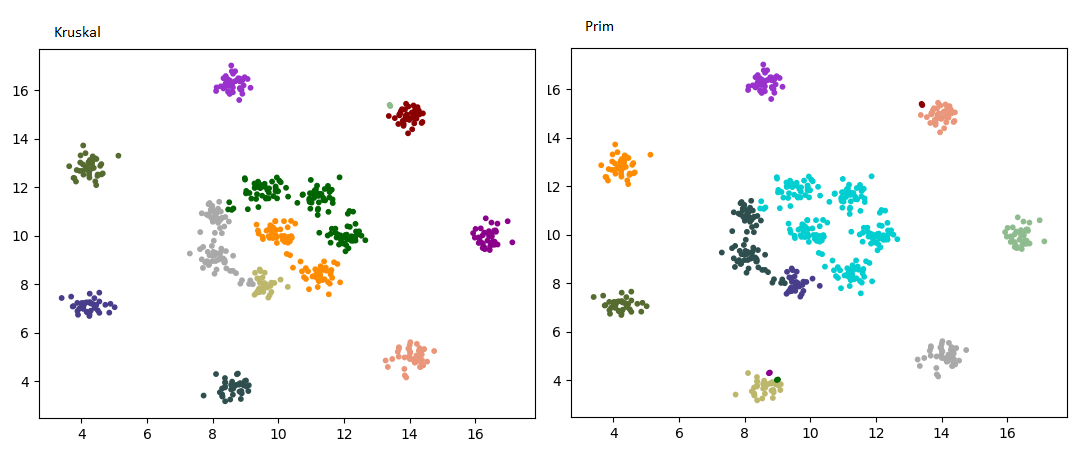
\includegraphics[scale=.5]{graficos/r15.png}
 Fijamos $\sigma_{T}$ $=$ 3.3 y $f_{T}$ $=$ 2.4, d = 2. Por razones de espacio evitamos poner a Kruskal sin path compression porque dan exactamente lo mismo.
 Los valores de los parametros fueron: factor de proporción en 1.8 y la desviación en 3.8. En este caso, pequeñas modificacione en el factor de proporción o desviación no generaban clusters diferentes. Sin embargo se puede apreciar cómo los clusters exteriores están definidos muy parecida a cómo sería esperable mientras que en el centro empiezan a juntarse puntos de -a nuestra percepción- diferente cluster. El problema es que al mirar con atención los posibles ejes que unen en el AGM los nodos que serían de diferente cluster cumplen ciertas cosas:
\begin{center}
 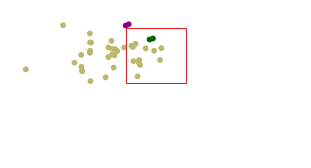
\includegraphics[scale=.7]{graficos/r15_zoom.png} 
 
\end{center}
Si hacemos un zoom a la zona del cluster marrón claro de Prim que tiene como dos clusters adicionales y no intuitivo para nuestra percepción, demarcamos la zona marcada con rojo y obsvervamos el caso del cluster verde es bastante visible que cualquier de los posibles ejes que los une (a los nodos) en el AGM va a cumplir tener mayor factor de proporción de promedio con respecto a los vecinos. Respecto de la desviación podría justificarse de un modo similar. Entonces podemos justificar de forma mas o menos razonable por qué se consideran - y bien- inconsistentes para nuestro modelo.
\\
Modifiquemos ahora un poco la forma de clusterizar. Fijemos d = 3, porque en este caso tiene sentido pensar que nos va a dar un poco de mayor consistencia en las mediciones, y utilicemos sólo la proporción entre ejes con $f_{T}$ $=$ 2.6.
\begin{center}
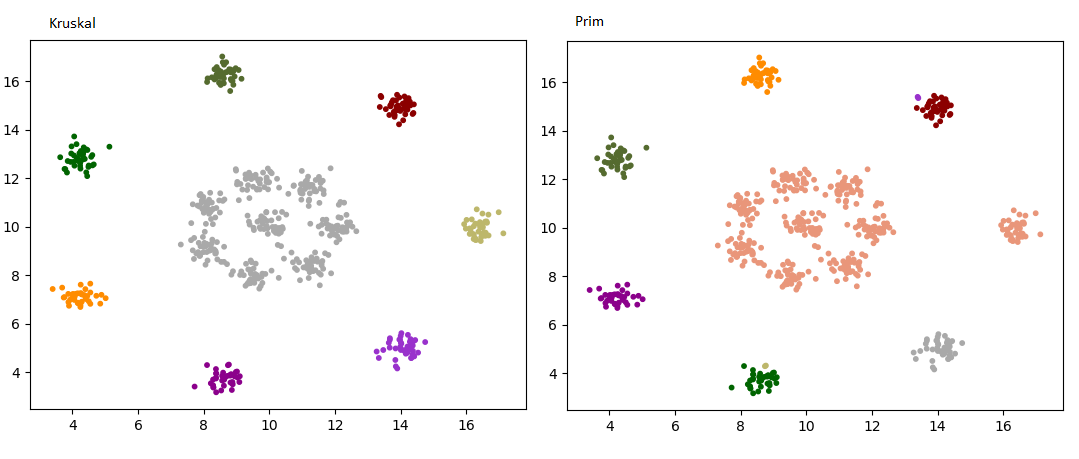
\includegraphics[scale=.5]{graficos/r15_2.png}
\end{center}
Como era esperado, el centro ahora se convierte en todo un gran cluster. Era algo esperado al agrandar los vecindarios, porque de esa manera por la densidad y distribución de los puntos de centro tiene sentido pensar que al tener en cuenta más vecinos será más complicado superar los 2.6 de proporción de eje. Si llegaramos a reducir el valor, es posible que obtengamos clusters no tan representantivos porque al sacar la desviación de consideración estamos sacando información útil para decidir si separar dos conjuntos de puntos más alla si existe algún eje lo 'suficientemente' largo.
\begin{center}
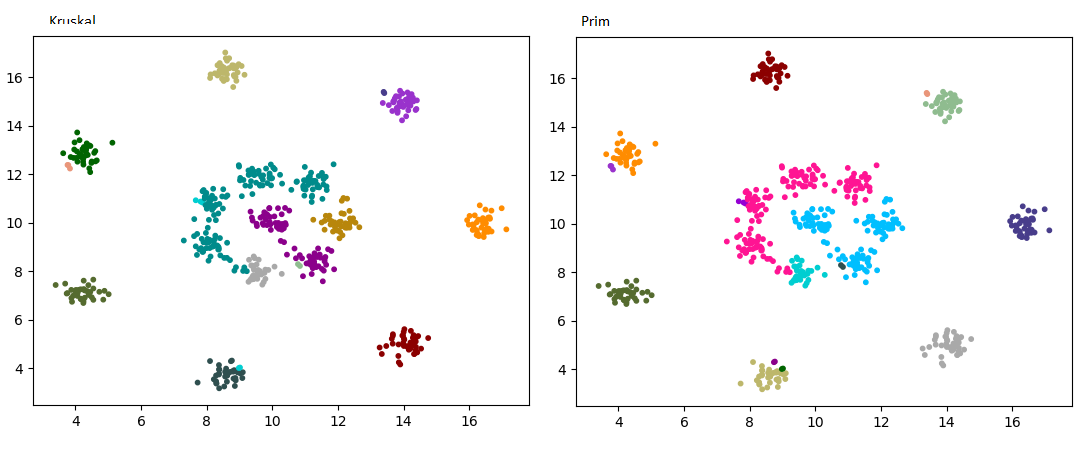
\includegraphics[scale=.5]{graficos/r15_3.png}
\end{center}
Efectivamente podemos ver que se encuentran más clusters debido a que como dijimos hay menos información con la cuál decidir, es decir, quizá dos nodos están suficientemente alejados pero por la dispersión de vecinos que tienen a nuestros ojos forman parte de lo mismo.\\
Para cerrar este tipo de contextos, encontramos que al igual que antes, Prim suele tender a generar clusters 'aislados' que intentaremos dar explicar viendo más casos y recopilando más información.
\\



\subsection{Dataset: Spiral}
\subsubsection{Tiempos}
\begin{table}[ht]
\caption{Tiempos de ejecución en milisegundos} % title of Table
\centering % used for centering table
\begin{tabular}{c c c c} % centered columns (4 columns)
\hline\hline %inserts double horizontal lines
Cant.Puntos & Kruskal & Kruskal sin path comp & Prim \\ [0.5ex] % inserts table
%heading
\hline % inserts single horizontal line
312 & 33 & 32 & 32.66 \\ [1ex] % [1ex] adds vertical space
\hline %inserts single line
\end{tabular}
\label{table:nonlin} % is used to refer this table in the text
\end{table} 


\begin{figure}[!htb]
   \begin{minipage}{0.45\textwidth}
     \centering
     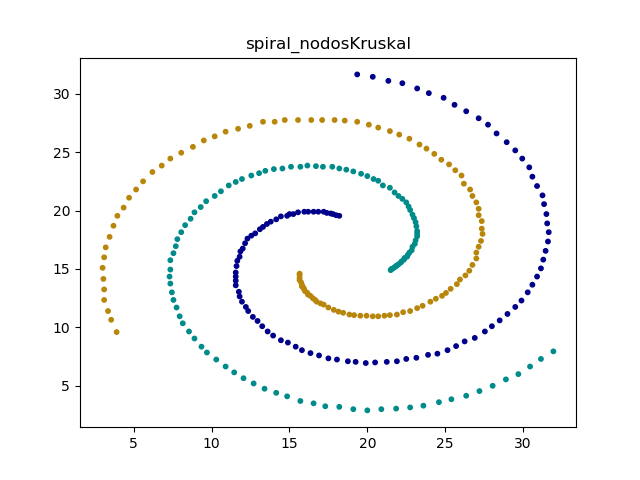
\includegraphics[scale=.5]{graficos/spiral_nodosKruskal.png}
   \end{minipage}\hfill
   \begin{minipage}{0.45\textwidth}
     \centering
     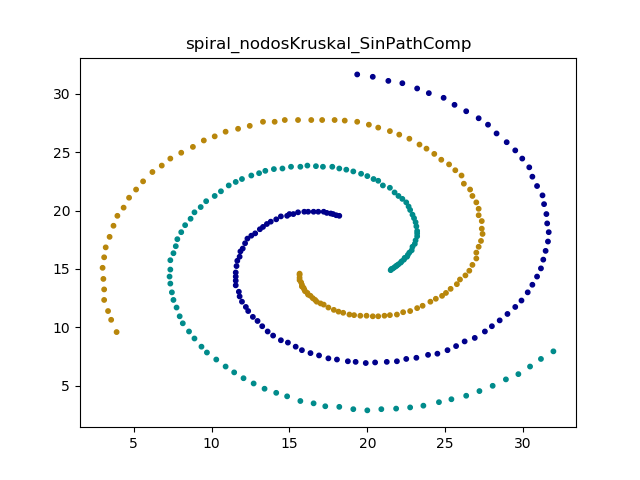
\includegraphics[scale=.5]{graficos/spiral_nodosKruskal_SinPathComp.png}
   \end{minipage}\hfill
   
\end{figure}

\subsubsection{Gráficos}
En este caso fijamos $f_{T}$ $=$ 3.3 y la profundidad del vecindario la fijamos en 2 y 3. Es razonable pensar que ambos AGM serán similares porque no hay demasiadas opciones de ejes para los nodos, porque cada una de las líneas de puntos tiene pocos vecinos cercanos (si pensamos en el grafo completo) con los cuales tiene sentido que se una formando una distancia mínima. Imaginemos el grafo completo y su conversión a AGM y pensemos que entre cada una de las líneas de puntos que vemos como clusters diferente existe una arista que las une (por ser un árbol) y si habría más de una seguro se podría encontrar un árbol generador con menor peso y esto sería absurdo porque Kruskal y Prim nos garantizan que lo consiguen, de modo que tiene sentido pensar que entre cada una de esas líneas existe sólo una arista que las une y que su peso es mucho mayor al de cualquiera de los demás ejes. Entonces al momento de experimentar, pensar en la profundidad de vecinos o proporción de eje inconsistente desde el detalle no tiene gran sentido, dado este caso donde las líneas están bien separadas no hay problemas para conseguir una separación de nodos intuitiva. \\


\subsection{Dataset: Pathbased}

\subsubsection{Tiempos}
\begin{table}[ht]
\caption{Tiempos de ejecución en milisegundos} % title of Table
\centering % used for centering table
\begin{tabular}{c c c c} % centered columns (4 columns)
\hline\hline %inserts double horizontal lines
Cant.Puntos & Kruskal & Kruskal sin path comp & Prim \\ [0.5ex] % inserts table
%heading
\hline % inserts single horizontal line
300 & 32 & 46 & 27 \\ [1ex] % [1ex] adds vertical space
\hline %inserts single line
\end{tabular}
\label{table:nonlin} % is used to refer this table in the text
\end{table} 

\subsubsection{Gráficos}
En este caso, tenemos algo similar al anterior pero tenemos una distribución de puntos que nos hace pensar que probablemente sea más dificil de encontrar una clusterización clara y tengamos que ajustar las desviaciones, el vecindario, y las proporciones de peso entre ejes. clusterización clara. 
\begin{center}
     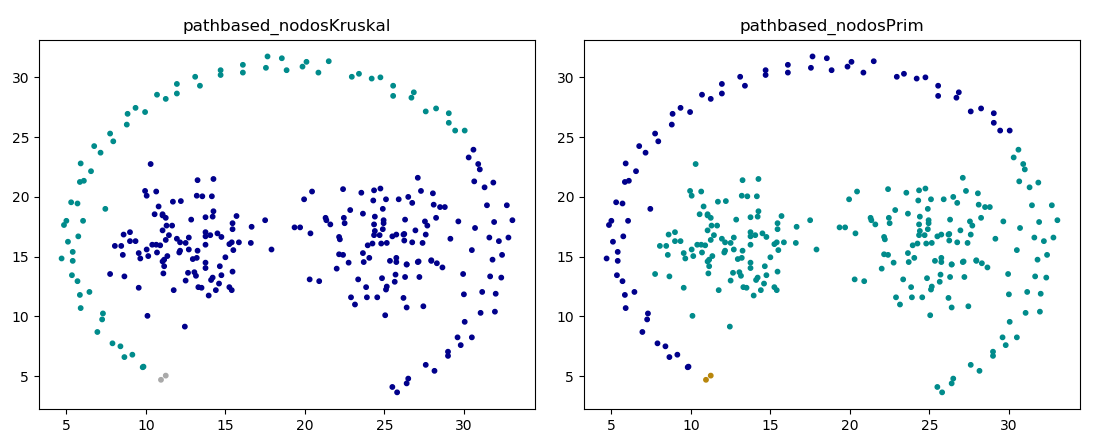
\includegraphics[scale=.5]{graficos/pathbased_nodosKruskal_nodosPrim.png}
\end{center}

Como vemos, fijando $f_{T} = 2.35$, d $=$ 3, lo que conseguimos no es lo que esperaríamos ver clusterizado. Es otro caso en donde la distribución de los puntos, la cercanía entre los clusters esperables, la relación con los pesos de los ejes del grafo, entre otras cosas, hacen que sea necesario trabajar un poco más para poder conseguir algo mejor.

\begin{center}
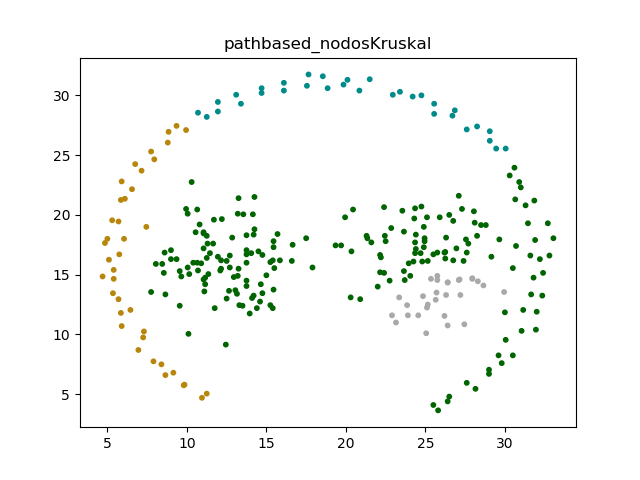
\includegraphics[scale=.5]{graficos/pathbased_nodosKruskal3.png}
\end{center}
Incluyendo ahora la desviación y ajustando un poco más los parámetros con $f_{T} = 1.9$, $\sigma_{T} = 2.5$ y d $=$ 2 tenemos algo que nos da más información para analizar.
Para que sea más fácil de ver lo señalamos en rojo y con un zoom a la imagen. Siempre es importante tener en la cabeza el posible AGM y a partir de ello analizar las razones por las que hay separaciones inesperadas de cluster.

\begin{center}
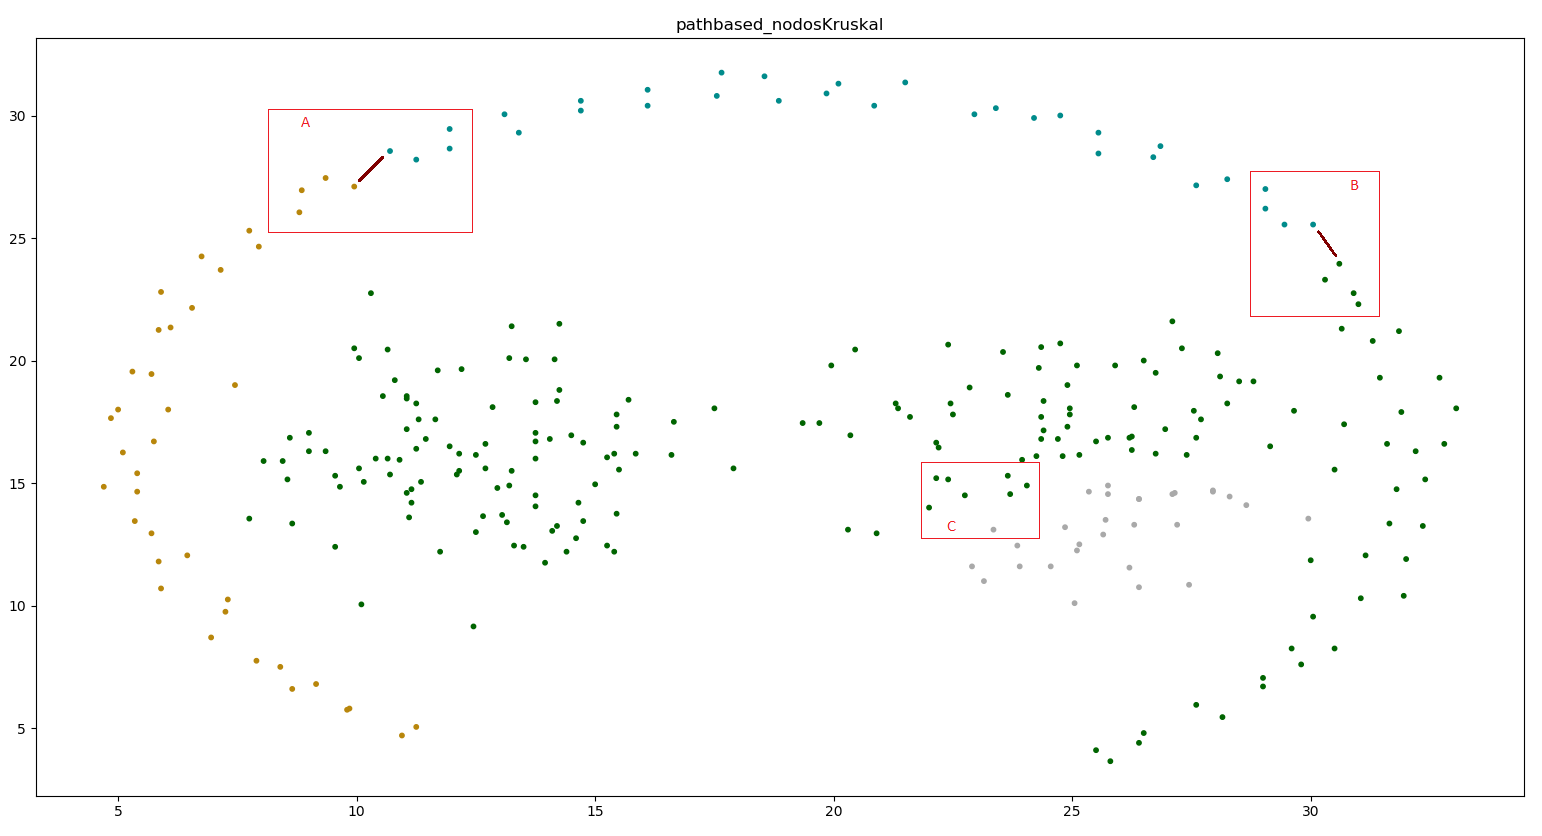
\includegraphics[scale=.41]{graficos/pathbased_nodosKruskal2.png}
\end{center}
El tema es claro: reducir el coeficiente de proporción de pesos nos genera clusters no esperados pero que si los analizamos en particular son correctos según nuestra medición. En las zonas señalizadas pusimos un eje bordo que simboliza la posible unión de los nodos en el AGM. Es claro que ese eje en proporción a los vecinos es superior y que para poder 'estabilizarlo' (en términos de evaluarlo y clusterizarlo como nosotros lo vemos) habría que tomar un vecindario más grande, posiblemente con d igual a 4 ó 5. En la zona C pasa algo similar y se le agrega algo: la distribución de puntos es diferente, lo cual genera que este tipo de situaciones sean difíciles de separar.


\subsection{Dataset: A1}
\subsubsection{Tiempos}
\begin{table}[ht]
\caption{Tiempos de ejecución en milisegundos} % title of Table
\centering % used for centering table
\begin{tabular}{c c c c} % centered columns (4 columns)
\hline\hline %inserts double horizontal lines
Cant.Puntos & Kruskal & Kruskal sin path comp & Prim \\ [0.5ex] % inserts table
%heading
\hline % inserts single horizontal line
3000 & 3839.66 & 5934.33 & 1939.33 \\ [1ex] % [1ex] adds vertical space
\hline %inserts single line
\end{tabular}
\label{table:nonlin} % is used to refer this table in the text
\end{table} 

\subsubsection{Gráficos}
En este caso tenemos una clusterización bastante evidente a simple vista sin embargo después de variar los parámetros lo más parecido que podemos conseguir es lo siguiente:
\begin{center}
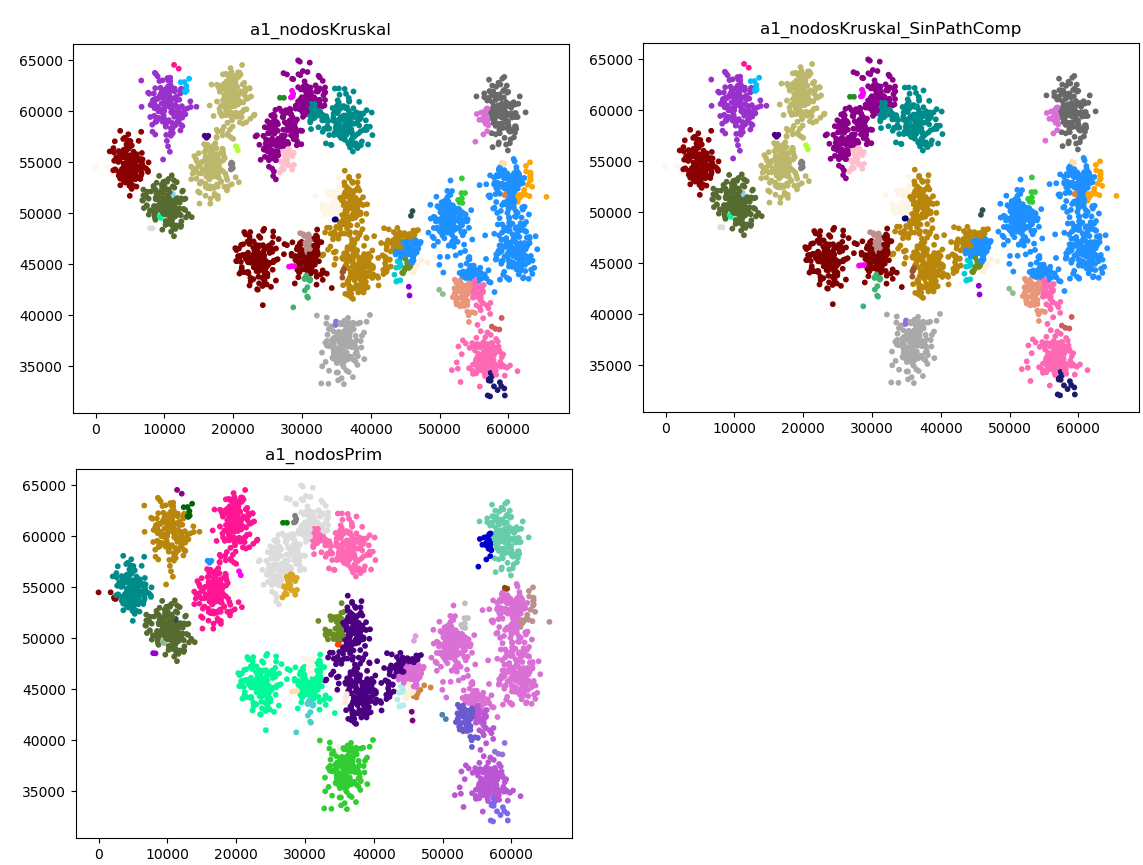
\includegraphics[scale=.41]{graficos/a1_nodosKruskal_Prim.png}
\end{center}
Volvemos a encontrar un factor que se viene repitiendo en los distintos datasets: la transición entre lo que a simple vista son diferentes clusters algorítimicamente no suele ser fácil de detectar. Modificando los parámetros podemos llegar a solucionar el problema en alguna zona en particular y al mismo romper lo anteriormente bien -a nuestra percepción- clusterizado. Un posible camino sería subdividir las áreas de puntos que queremos clusterizar y separarlas en función de patrones similares que permitan fijar los parámetros sin romper otras zonas ysa clusterizadas. Sin embargo en este caso en particular no es muy claro qué áreas subidividir.\\
Veamos otro caso en donde sería un poco más claro cómo dividir en caso de que pase esto.

\subsection{Dataset: Compound de Zahn}
\subsubsection{Tiempos}
\begin{table}[ht]
\caption{Tiempos de ejecución en milisegundos} % title of Table
\centering % used for centering table
\begin{tabular}{c c c c} % centered columns (4 columns)
\hline\hline %inserts double horizontal lines
Cant.Puntos & Kruskal & Kruskal sin path comp & Prim \\ [0.5ex] % inserts table
%heading
\hline % inserts single horizontal line
399 & 61 & 90.33 & 46 \\ [1ex] % [1ex] adds vertical space
\hline %inserts single line
\end{tabular}
\label{table:nonlin} % is used to refer this table in the text
\end{table} 
\subsubsection{Gráficos}
Fijando $f_{T} = 1.19$, d $=$ 2, $\sigma$ $=$ 4.3 encontramos lo siguiente: (por motivos de espacio y que los 3 AGM dan igual sólo ponemos 1)
\begin{center}
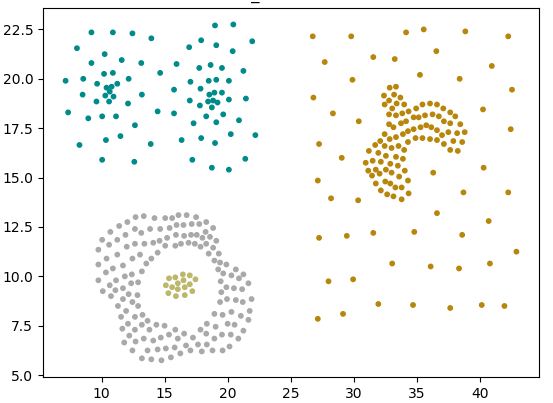
\includegraphics[scale=.6]{graficos/zahn.png}
\end{center}
Es claro que la clusterización obtenida está cerca de la esperada, aunque también sería esperable que los de la esquina superior izquierda sean dos diferentes y que el de la derecha también lo sea. Primero vamos a tratar de modificar los parámetros para obtenerlo y si no podemos vamos a intentar aplicar clusterizar por partes, porque acá sí es más claro que tenemos tres zonas que podemos tratar por separado.
\begin{center}
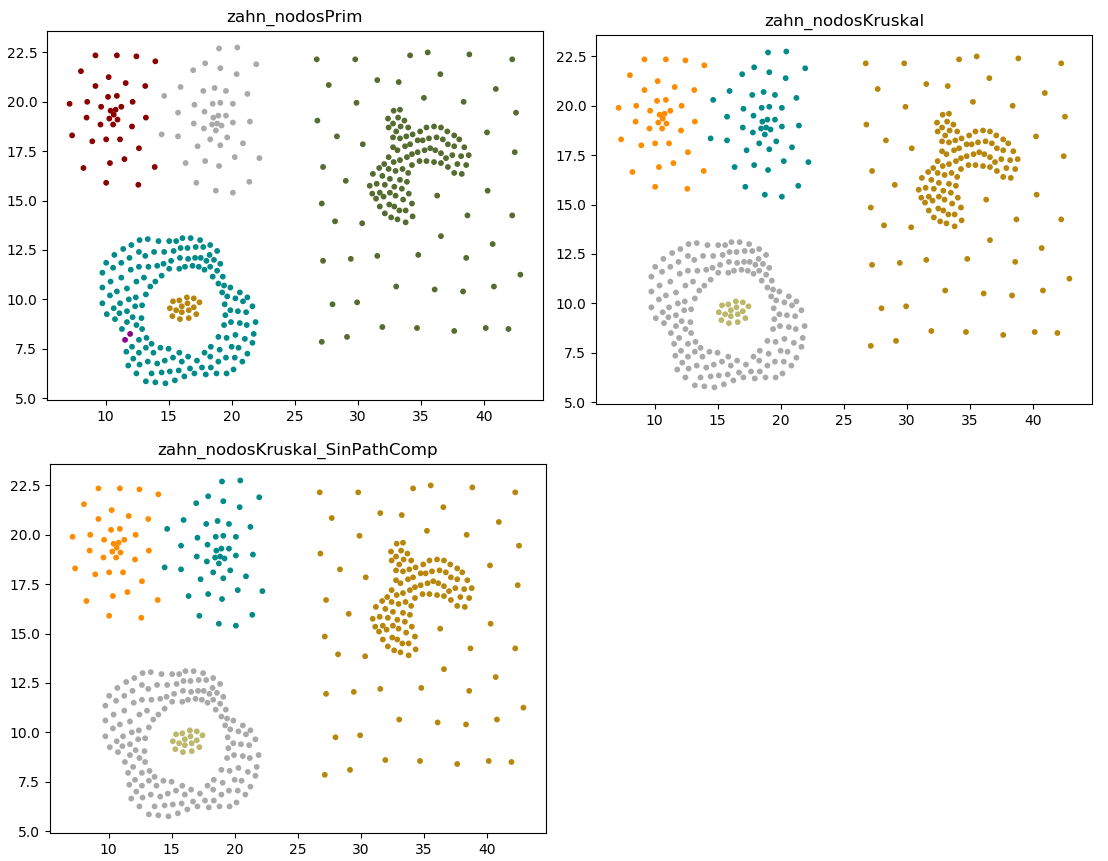
\includegraphics[scale=.55]{graficos/zahn_nodosPrim_Kruskal.png}
\end{center}
Si  miramos con atención, la solución que utiliza Prim generó un cluster adicional, mientras que Kruskal no, aunque ninguno pudo clasificar en dos la parte derecha de la imagen.\\
Intentemos probar ahora clusterizar esa parte sola, tomando a partir de x $>=$ 25 y ver si podemos clusterizarla y en cierto modo terminar clusterizar 'bien' todo el gráfico.
\begin{center}
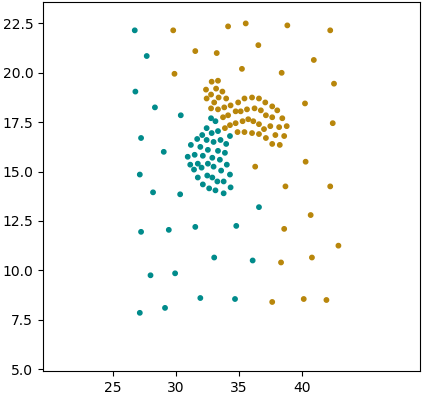
\includegraphics[scale=.6]{graficos/zahn_nodos2.png}
\end{center}
Obtuvimos está nueva clusterización fijando d $=$1, $\sigma$ $=$ 1.2, $f_{T}$ $=$ 1.2, y nuevamente nos encontramos con dificultades para poder separar grupos de puntos que sacándolos del contexto anterior parecía bastante sencillo de separar, los Gestalts principles se hacen presentes en casi todos los experimentos.\\

Retomando el gráfico anterior donde Prim generaba un cluster adicional a Kruskal, lo que hicimos fue hacer un zoom en esa región y análisis en detalle, marcando en rojo cuáles son las aristas que unen esos nodos en particular. Obtuvimos lo siguiente:
\begin{center}
\includegraphics[scale=.6]{graficos/zahn_conex_Prim.png}
\includegraphics[scale=.6]{graficos/zahn_conex_Kruskal.png}
\end{center}

Ambos métodos tienen diferentes técnicas para generar un AGM, esto es algo que no podemos controlar en profundidad en todos los datasets pero que en este en particular notamos, aunque es posible que en otros también ocurriese y no se notara porque no afectaba a la clasificación de los nodos. En este caso sí y se nota claramente en la imagen. Internamente, la arista en cuestión es la número 280 en Kruskal mientras que Prim la consiguió como arista 115. En Prim imaginamos que esta parte es la especie de 'hojas' del árbol y que la raíz está hacia la derecha. Marcamos con azul la arista que se considera inconsistente. En Kruskal aparentemente sería una situación inversa, estamos donde sería algo similar a la raíz y hacia el otro lado estaría esta situación. En la imagen es apreciable que al cambiar esas relaciones el vecindario también es diferente y en la zona que une Kruskal aumentan levemente los promedios de pesos de ejes y esto impide que sea considerado inconsistente.


\subsection{Conclusiones}
Durante la experimentación con diferentes tipos de conjuntos pudimos comprobar en persona las discusiones que tuvieron lugar en secciones previas de la introducción teórica. Vimos cómo son afectados los análisis en función de pequeños movimientos de los parámetros y la dificultad para encontrar una configuración que permita una clasificación cercana a nuestra percepción en todo su conjunto. En caso de tener que clusterizar diferentes gráficos se deberá necesariamente contar con el tiempo para una experimentación exhaustiva que permita realizarlo y en muchos casos la subdivisión de los gráficos para el tratado de zonas que presenten patrones de caracterización diferentes y estar preparados para no conseguir los clusters idénticos a lo esperado. 
\\ También cabe mencionar las diferentes técnicas de generación de AGM, donde por lo menos a nivel clusterización no hubo una diferencia considerable para alguno en la clusterización de algún conjunto en particular. Sí hay que mencionar las diferencias de performance evaluadas: es claro que más alla de la complejidad teórica Kruskal con path compression en la práctica es mucho mejor y en algunas situaciones es más notable que en otras. Además, en este trabajo en particular se construyó el AGM partiendo del grafo completo, lo que quiere que decir que una técnica como Kruskal en la que es necesario ordenar las aristas se ve altamente perjudicada. Otras forma consisten en calcular un grafo con los k-vecinos más  cercanos para cada nodo y de esta forma evitar partir de un grafo completo en donde m $\approx$ $n^{2}$.\\ En general, clusterizar en determinados casos requerirá aceptar cierto grado de error, debido a la falta de comprobación exacta de los resultados, y el contexto determinará cuán exacto y exhaustivo, respecto de una percepción esperada, deberán ser los métodos considerados para la clusterización.


\pagebreak

%Acá va todo lo que hicieron Dylan y Gabi.
%\section{Arbitraje}
%\section{Justificación teórica}
%\section{Algoritmos presentados}
%\subsection{Complejidad}
%\section{Experimentación}

\section{Arbitraje}

En el mundo de la finanzas se denomina $arbitraje$ al hecho de comprar y vender un recurso de manera simult\'anea para generar una ganancia, aprovech\'ose de los desbalances de los precios en diferentes mercados. La idea es que al ser operaciones simult\'aneas el abitrajista no corre riesgo en sus transaccciones. En genewral, los desbalances necesarios para darse una situaci\'on de arbitraje provienene de desincronizaciones de los mercados.
\\

Supongamos que hay un recurso $R$ disponible para vender y comprar en los mercados $M_{1}$ y $M_{2}$. En $M_{1}$ nos dan 36.80 pesos por vender u na unidad de $R$ u nos cuesta 37.50 pesos comprar un a unidad. En $M_{2}$ en cambio nos dan 36.90 pesos por vender una unidad  de $R$ y nos cuesta 37.65 pesos comprar una unidad. En este caso no existe oportunidad de arbitraje. No hay gorma con estos dos mercados que vendamos y compremos unidades del recurso $R$ y generemos una ganancia. Sin embargo, en un determinado momento del d\'ia sucede un evento que valoriza el recurso $R$. $M_{1}$ se entera de este suceso y actualiza sus cotizaciones. Luego de este cambio nos dan 37.67 pesos por v ender una u nidad de $R$ y nos cuesta 39.95 pesos comprar una unidad. Las noticias llegan m\'as tarde a $M_{2}$ por lo que todav\'ia no se enter\'o del suceso que valoriz\'o a $R$, por los que sus precios siguen intactos por un per\'iodo m\'as. En este caso s\'i existe oportu nidad de arbitraje.  Podemos simultaneamente comprar varias unidades del recurso $R$ en $M_{2}$ y vender varias unidades en $M_{1}$. De esta manera, por cada unidad que se compra/vende estamos obteniendo 0.02 pesos sin ning\'un tipo de riesgo.
\\

Afortunadamente, este situaci\'on, esta situaci\'on no es algo que suceda a menudo. De hecho, en el caso que suceda, muchas veces no incluye un \'unico recurso sino que involucra a varios recursos en varios mercados distintos.
\\

En este problema lo que nos gustar\'ia es si existe oportunidad de arbtiraje entre varias divisas (Pesos, D\'olares, Libras, Reales, Bitcoins, etc.). Para eso contamos con la tasa de cambio entre cada par de divisas. En caso de existir arbitraje, queremos saber qu\'e divisas son involucradas en el proceso.
\\

A continuaci\'on se expondr\'an algunos ejemplos, cada uno con su respectiva soluci\'on en caso de existir, para poder entender mejor el problema.
\\

\noindent{\large $\textbf{Ejemplo No. 1:}$} 

Para el primer ejemplo tomaremos las divisas:
\begin{itemize}
    \item[•] $d_{0}$ = D\'olares estadounidenses.
    \item[•] $d_{1}$ = Pesos argentinos.
    \item[•] $d_{2}$ = Euro.
    \item[•] $d_{3}$ = Libra esterlina.
\end{itemize}

y la "matriz de cambios" conformada por el peso de los ejes:

\[
M=
  \begin{bmatrix}
    1 & 36,64 & 0,863 & 0,760 \\
    0,027 & 1 & 0,023 & 0,020 \\
    1,159 & 42,42 & 1 & 0,88 \\
    1,315 & 48,20 & 1,136 & 1 \\
  \end{bmatrix}
\]

En la que tomaremos estos pesos como los factores multiplicativos para pasar del valor de un nodo a otro, por eso cada nodo tendr\'a distancia 1 de si mismo, entonces, si observamos el grafo asocidado a la matriz, podemos ver que este ser\'a un pseudografo dirigido completo. Ser\'a completo ya que cada divisa tendr\'a que tener un valor de cambio para otra divisa.

En resumen: $m_{i,j}$ ser\'a lo que tenga que multiplicar el valor de lo que tenga en la divisa $d_{i}$ para pasar a la divisa $d_{j}$.

El grafo asociado a nuestra matriz ser\'a:

\begin{figure}[h]
\centering 
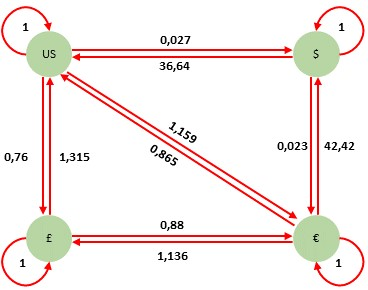
\includegraphics{Grafoejemplo2.jpg}
\end{figure}

Para que nuestro problema tenga soluci\'on debemos encontrar al menos un ciclo de divisas tales que al volver a la divisa de la que empezamos haya arbitraje.

Y, si probamos con un ciclo que empieze con  el dolar tenemos los siguientes resultados:
\begin{itemize}
    \item[•] Si el ciclo es {$d_{0}$,$d_{1}$,$d_{0}$} es decir (d  \'olares-pesos-d\'olares) tenemos que al regresar nuestra divisa valdra 1*36,64*0,027 de lo que val\'ia en un principio, es decir 0,9893 por lo tanto no se producir\'a arbitraje.
    \item[•] Si el ciclo es {$d_{0}$,$d_{2}$,$d_{0}$} es decir (d  \'olares-euros-d\'olares) tenemos que al regresar nuestra divisa valdra 1*0,863*1,159 de lo que val\'ia en un principio, es decir 1,0002: 2 diezmilesimas m\'as que antes, por lo cual aqu\'i si se producir\'a arbitraje
\end{itemize}

Como pude encontrar al menos un ciclo de divisas que me generara arbritraje, mi soluci\'on ser\'a: $d_{0}$,$d_{2}$,$d_{0}$.
\\

\noindent{\large $\textbf{Ejemplo No. 2:}$}

Para el segundo ejemplo se considerar\'a un caso en particular: cuando las divisas tienen el mismo valor de cambio entre todas. Es decir, al pasar de una moneda a otra esta sigue valiendo lo mismo. La matriz correspondiente al caso actual con 3 divisas ser\'a

\[
M=
  \begin{bmatrix}
    1 & 1 & 1 \\
    1 & 1 & 1 \\
    1 & 1 & 1 \\
  \end{bmatrix}
\]

y su pseudografo asociado
\begin{figure}[h]
    \centering
    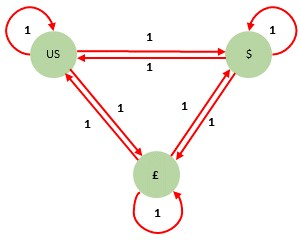
\includegraphics{Grafoejemplo1.jpg}
\end{figure}


En este caso se puede observar que ning\'un ciclo de divisas podr\'a generar alg\'un tipo de ganancia, ya que al pasar por cualquier divisa y volver a la divisa inicial esta conservar\'a su valor original, de manera que no habr\'a ganancia, pero tampoco p\'erdida. Por lo tanto podremos concluir que  no existir\'a oportunidad de arbitraje.
\\

\noindent{\large $\textbf{Ejemplo No. 3:}$}

Como \'ultimo ejemplo tendremos en cuenta el grafo en el cual $\forall$ divisa $d_{i}$ con 0 $\leq i \leq$ 3 exista un ciclo de divisas que empieza y termina en $d_{i}$ tal que haya posibilidad de arbitraje. Es decir, si tenemos la matriz
\[
M=
  \begin{bmatrix}
    1 & 1.41 & 3.14 & 1.6180 \\
    1.01 & 1 & 2,02 & 3,03 \\
    4 & 4 & 1 & 4 \\
    1.03 & 1.06 & 1.09 & 1 \\
  \end{bmatrix}
\]


Y como podemos notar seg\'un lo mencionado previamente, habr\'a  soluci\'on posible al problema y ser\'a m\'as de una. Es decir, tomando los valores de cambio, cualquier ciclo de la forma C = \{$d_{i}, d_{j},....,d_{i} \}$ cumplir\'a que genere arbitraje ya que todas las divisas ya sea para la ida o para la vuelta tienen una ganancia al realizar cualquier cambio debido a que todas las aristas que unen divisas son mayores a 1. Y como el problema se trata de responder si existe posibilidad y devolver alguno de estos ciclos, podremos devolver cualquiera de ellos y esa ser\'a la soluci\'on.
\pagebreak
\section{\huge Algoritmos y soluciones}

En la presente secci\'on se explicar\'a la idea detr\'as de cada algoritmo, como la justificaci\'on de la complejidad de cada uno. Se usar\'a pseudoc\'odigo para explicar los mismos.


Para la resoluci\'on de nuestro problema utilizaremos las siguientes definiciones:
\\

{\large $\textbf{Definicion:}$} el $\textbf{camino m\'inimo}$ entre dos vértices (o nodos) es aquel camino tal que la suma de los pesos de las aristas que lo constituyen es mínima respecto de otros caminos.
\\

{\large $\textbf{Definicion:}$} el $\textbf{Circuito M\'inimo Multiplicativo }$ de un nodo v ser\'a aquel que cumpla lo siguiente:

Si de avanzar por el camino que inicia en v, multiplicando por los factores multiplicativos(pesos de las aristas), al finalizar , se consiguiera volver a v con un valor menor al inicial, este se considerara un $\textbf{Camino M\'inimo Multiplicativo }$


Entonces, en nuestro problema, diremos que habr\'a soluci\'on si al aplicar nuestros algoritmos, al regresar por alg\'un circuito, el resultado del circuito m\'inimo de un nodo a s\'i mismo es mayor que 1.

Para la resoluci\'on del problema consideraremos dos opciones/variantes, las cuales utilizaran cada una la idea de un algoritmo de camino m\'inimo conocido.

\subsection{Primer Aproximaci\'on (Bellman-Ford)}
\subsubsection{El Algoritmo}

Para la presente aproximaci\'on del problema se tendr\'a en cuenta el algoritmo de Bellman-Ford con algunas modificaciones a fin de ser \'util con el problema de arbitraje.

    Normalmente este algoritmo se usa para calcular los caminos m\'inimos de un nodo en espec\'ifico hacia todos los nodos en un grafo. En nuestro caso, no queremos calcular eso sino alg\'un $\textbf{Camino M\'inimo Multiplicativo}$ que haya en el grafo. Por lo tanto se usar\'an las herramientas de detecci\'on presentes en el algoritmo original y la idea general del mismo para poder devolver el ciclo de divisas que genera el arbitraje. Es decir, como este algoritmo calcula el camino m\'inimo, si cambiaramos las sumas por multiplicaciones podr\'iamos calcular el camino m\'inimo multiplicativo. Y en este caso, lo que haremos es cambiar el menor por un mayor y lo que obtendremos por el algoritmo ser\'a un camino multiplicativo que "maximice".

Para facilitar la comprensi\'on del mismo se introducir\'a el pseudo-c\'odigo del algoritmo que resuelve una parte intermedia del problema.
\begin{Verbatim}[commandchars=\\\{\}]
BellmanFordArbitraje(M, s)
    n = rows(M)
    distancias(n, -INFINITO)
    padre(n, -1)
    ciclo = vacio()
    distancias[s] = 1
    cambio = true
    finished = false
    
    for(int k = 1; k < n+1 && cambio && !finished; k++)
        cambio = false
        for(int i = 0; i < n && !finished; i++)
            for(int j = 0;j < n && !finished; j++)
                \textcolor{red}{if distancias[i] * M[i][j] > distancias[j]:}
                    cambio = true
                    distancias[j] = distancias[i] * M[i][j]
                    padre[j] = i
                    if distancias[s] > 1: finished = true
                
            
    if (!cambio || distancias[s] <= 1)
        return ciclo

    comienzoCiclo =  s;
    current = comienzoCiclo
    agrego current a ciclo
    mientras current != comienzoCiclo
        agrego current a ciclo
        current = padre[current]
    agrego current a ciclo
    return ciclo
\end{Verbatim} 

Para explicar el funcionamiento de este algoritmo se tendr\'a en cuenta la utilidad de las siguientes variables:
\begin{itemize}
    \item[•] distancias: en la posicion s se guardar\'a la distancia del nodo s a s\'i mismo por alg\'un camino/ciclo.
    \item[•] padre: se utilizar\'a para reconstruir el ciclo que involucre a s en caso de exitir uno.
    \item[•] tanto cambio como finished ser\'an flags que servir\'an para terminar antes con el triple ciclo.
    \item[•] ciclo: ser\'a el ciclo que genere el arbitraje empezando desde la divisa s.
\end{itemize}
Con todo lo anteriormente dicho, podemos empezar a explicar el funcionamiento del algoritmo:

Si observamos el triple ciclo for, podemos ver que este se parece un poco al del algoritmo de Bellman-Ford sobre Matrices de Adyacencia, con las siguientes diferencias:

-En la versi\'on original el for m\'as interno de todos solo itera sobre los vecinos de i, pero en particular, como todas las divisas se pueden intercambiar entre si, el grafo ser\'a completo y los vecinos de i ser\'an todos los nodos.

-Al igual que en Bellman-Ford usaremos la idea de relajar ejes y reemplazar valores en caso de encontrar un camino mejor utilizando el nodo i como intermediario, la diferencia en este caso ser\'a que la distancia de un nodo a s\'i mismo tambien podr\'a mejorar, y esto ser\'a lo que ocurra en caso de existir posibilidad de arbitraje: Se encontr\'o un camino (en este caso ciclo) que al pasar por cierta/s divisa/s genere un valor mayor al que se encontraba originalmente. Es decir, de relajar ejes tambi\'en podr\'a resultar que la distancia de un nodo a si mismo mejore, cosa que no ocurre en el algoritmo original para caminos m\'inimos, (salvo que hayan ciclos negativos) y con mejor en este caso nos referimos a que aumente. Dicho esto podemos observar que el ciclo de divisas (empezando y terminando en s) que genere arbitraje ser\'a identificado en el triple ciclo de nuestra funci\'on intermedia mediante el mecanismo de padres. Una vez terminada la "identificaci\'on" ya sea por que hizo todas las iteraciones o por el valor de alguna flag, se proceder\'a a armar dicho ciclo.


Como se mencion\'o antes, padre servir\'a para reconstruir el ciclo que genere arbitraje luego de ejecutar este triple ciclo. Notar que los flags mencionados previamente cumplir\'an con las siguientes funciones espec\'ificas:
\begin{itemize}
    \item[•] cambio ser\'a el encargado de verificar que el vector de distancias cambie por cada iteracion en k, de  no ocurrir esto el ciclo terminar\'a. Esto nos garantizar\'a que nuestra implementaci\'on sea la optimizada, en la cual no se realizar\'an iteraciones de m\'as. Si bien esto no altera la complejidad te\'orica, ayudar\'a en cuanto a la complejidad pr\'actica.
    \item[•] finished al igual que cambio ayudar\'a a reducir la cantidad de iteraciones en caso de ocurrir lo siguiente: si la distancia del nodo s a si mismo es mayor a 1. ¿Y por qu\'e esto sirve? Simple, esto lo que nos quiere decir es que el algoritmo encontr\'o alg\'un ciclo que empieza y termina en s por lo tanto no es necesario seguir buscando otro ciclo. Al igual que antes, esto no ayuda en cuanto a complejidad te\'orica pero si en cuanto a pr\'actica.
\end{itemize}


Por lo tanto podemos decir que el algoritmo servir\'a para calcular el problema de arbitraje si la divisa pasada por par\'ametro forma parte de un ciclo que aumente el valor al volver, el cual ser\'a el resultado. Es decir, si quisi\'eramos resolver el problema sin importar desde cu\'al nodo se comienza el ciclo deber\'iamos repetir la idea para todos los nodos, lo cual ser\'a realizado por la funci\'on ArbitrajeBF:

\begin{Verbatim}[commandchars=\\\{\}]
problemaArbitrajeBF(M)
    ciclo = vacio()
    n = M.rows()
    for int i = 0; i < n; ++i 
        ciclo = bellmanFordArbitraje(M, i)
        \textcolor{red}{Si ciclo no es vacio, salgo del for.}
            
    return ciclo
\end{Verbatim}

Notar tambi\'en que nuestro algoritmo devuelve el primer ciclo que encuentre, en caso de haber uno, empezando desde el nodo 0, lo cual puede verse en nuestro pseudo-c\'odigo en color rojo.

Como efectivamente realizamos esto para cada nodo (divisa) del grafo, y fue probado que resuelve el problema en particular para un nodo, podremos decir que nuestro algoritmo final resuelve el problema de \textbf{manera exacta} para cualquier divisa del grafo.

\subsubsection{An\'alisis de Complejidad}
Para nuestro an\'alisis de complejidad podremos reutilizar complejidades te\'oricas de los algoritmos subyacentes de camino m\'inimo que usamos para resolver los problemas. En particular, podemos ver que nuestro triple ciclo del algoritmo BellmanFordArbitraje tendr\'a complejidad $\mathcal{O}$($n^{3}$) como el del algoritmo original sobre matrices de adyacencias y que lo dem\'as (asignaciones, rearmar el ciclo) tendr\'a a lo sumo complejidad $\mathcal{O}$(n) por lo tanto podemos decir que:
\begin{center}
Complejidad Te\'orica de BellmanFordArbitraje: $\mathcal{O}$($n^{3}$)
\end{center}

Y como realizamos esto una vez por cada nodo en problemaArbitrajeBF, y siendo nuestro peor caso el de que el ciclo no exista o este exista pero est\'e en el nodo n-1, podemos concluir que la complejidad te\'orica de nuestra primer aproximaci\'on al problema ser\'a:
\begin{center}
T(n) = $\mathcal{O}$($n^{3}$)*n = $\mathcal{O}$($n^{4}$)
\end{center}

\subsection{Segunda Aproximaci\'on (Floyd-Warshall)}
\subsubsection{El Algoritmo}
La idea inicial es, igual que en el de Bellman Ford, intentar modificar el algoritmo de Floyd para que "en vez de sumar, multiplique".\\
El algoritmo de Floyd se basa en el concepto de que "si el camino más corto de A a B pasa por C, entonces la distancia de A a B es la distancia de A a C más la distancia de C a B".\\
Nosotros ahora queremos encontrar el CMM (Camino Mínimo Multiplicativo) por lo tanto queremos demostrar que "si el CMM de A a B pasa por C, entonces la DMM de A a B es la DMM de A a C multiplicada por la DMM de C a B".\\
Donde DMM = Distancia Mínima Multiplicativa que es la mínima distancia de multiplicando el peso de las aristas del CMM.\\
Supongamos que el CMM(A,B) pasa por C.\\
Tenemos el CMM(A,C) con $X$ aristas que llamaremos $H_i$ con $0 \leq i < X$.\\
Tenemos el CMM(C,B) con $Y$ aristas que llamaremos $Q_i$ con $0 \leq i < Y$. \\
Tenemos el CMM(A,B) con $Z$ aristas que llamaremos $P_i$ con $0 \leq i < Z$. \\
DMM(A,C) = $\prod\nolimits H_i$\\
DMM(C,B) = $\prod\nolimits Q_i$\\
DMM(A,B) = $\prod\nolimits P_i$\\
Queremos probar que DMM(A,B) = DMM(A,C) * DMM(C,B).\\
Esto es equivalente a $\prod\nolimits P_i$ = $\prod\nolimits H_i * \prod\nolimits Q_i$\\
También es equivalente a $\prod\nolimits P_i$ = $\prod\nolimits (H \cup Q)_i$\\
Por lo tanto queremos probar que $P = H \cup Q$\\
Suponemos que esto es falso y nos quedan 3 casos:\\
1) $P \subseteq H$ \& $P \nsubseteq Q$\\
2) $P \nsubseteq H$ \& $P \subseteq Q$\\
3) $P \nsubseteq H$ \& $P \nsubseteq Q$\\
Caso 1:\\
Si esto es verdad entonces tomamos en el tramo C-B del CMM(A,B) y va a contener una distancia $d$.\\
Si $d \leq DMM(C,B)$ es absurdo por definicion de DMM!\\
Si $d > DMM(C,B)$ entonces se puede reemplazar el tramo C-B del CMM(A,B) por CMM(C,B) y obtendríamos una longitud menor del circuito, lo que probaría, pero esto es absurdo porque este ya era el CMM por lo tanto tenía distancia mínima.\\
Caso 2:\\
Es análogo al Caso 1.\\
Caso 3:\\
Es como el caso 1 y 2 juntos.\\
\\
Por lo que queda demostrado por absurdo que $P = H \cup Q$.\\
Por lo tanto la idea del algoritmo de Floyd puede utilizarse para resolver el problema del CMM.\\
También vamos a cambiar la comparación para guardarnos los máximos en vez de los mínimos así podemos obtener facilmente el resultado del ejercicio ya que el objetivo es buscar un ciclo positivo.\\
Sería exactamente lo mismo si invertimos la matriz y ejecutamos el clásico algoritmo de mínimos. Pero esto nos ayuda a evitar errores de precisión al invertir la matriz.\\ 
\\
Ahora vamos a generar un pseudocódigo para analizar los cambios que tendrían que hacerse:

\begin{Verbatim}[commandchars=\\\{\}]
FloydWarshallModificado(M)
    padres = inicializar_padres()
    
    Poner diagonal de M en 1
    
    for k = 0; k < n; k++ 
        for i = 0; i < n; i++
            for j = 0; j < n; j++
                dt = distancias[i][k] * distancias[k][j]
                if distancias[i][j] < dt
                    distancias[i][j] = dt
                    padres[i][j] = padres[k][j]
                endif
            endfor
        endfor
    endfor
    
    Recorremos la diagonal para ver si alguno quedo mayor que uno:
        Reconstruimos el ciclo a partir de ese con la matriz de padres
        Si lo logramos: ganamos! encontramos un ciclo positivo.
        
    Invertimos el ciclo (porque lo reconstruimos al reves)
\end{Verbatim}

Así es la primera idea de como sería el algoritmo. Es un típico algoritmo de Floyd-Warshall, recorre todos los nodos y para cada uno, se fija para todas las distancias si alguna se puede mejorar haciendo pasar al camino por ese nodo. La única diferencia es que ahora estamos usando multiplicación en vez de suma para poder encontrar las DMM y cambiamos la comparacion para que ahora guarde los mayores asi encontramos el ciclo positivo.\\
Luego de correr Floyd-Warshall obtenemos la matriz de distancias y la matriz de padres, pero... y el problema?...\\
Para recordar: Tenemos que obtener el ciclo.\\
Por lo tanto tenemos que recorrer la matriz de distancias y fijarnos si es que algún elemento de la diagonal dio mayor que 1.\\
Nosotros empezamos con todos 1s en la diagonal, esto quiere decir que si alguno terminó mayor eso significa que hay un ciclo que lo hizo "mejorar" de su valor original para ir a sí mísmo.\\
Si encontramos uno de estos podemos recorrer la matriz de padres comenzando en ese nodo y hacia atras para encontrar todo el ciclo.\\
Puede suceder que cuando estás recorriendo hacia atras la matriz de padres, te encuentres con otro ciclo antes de volver al nodo inicial del ciclo que estás buscando, tomamos la decision de que si esto sucede vamos a tirar a la basura el ciclo que encontramos hasta ahora y seguir recorriendo nodos de la diagonal hasta encontrar el nodo inicial del ciclo más chico y así devolver ese.\\
Finalmente damos vuelta el ciclo obtenido ya que lo reconstruimos de atrás para adelante y lo devolvemos ya que es el resultado del ejercicio.\\
\\

\subsubsection{An\'alisis de Complejidad}
Al igual que en Bellman-Ford, podremos reutilizar la complejidad te\'orica del algoritmo subyacente, el cual es sabido es $\mathcal{O}$($n^{3}$), y diremos que esta ser\'a la complejidad final ya que despu\'es del triple ciclo no hay nada que tenga mayor complejidad. Es decir:

Complejidad del triple ciclo = $\mathcal{O}$($n^{3}$).

Complejidad de llenar la matriz distancias y rearmar el ciclo en caso de existir uno = $\mathcal{O}$($n^{2}$).

Por lo tanto podemos concluir:

Complejidad Total del algoritmo = $\mathcal{O}$($n^{3}$).

\pagebreak
\section{Experimentaci\'on, An\'alisis y Conclusiones}
\subsection{Experimento de Complejidad}
Para este experimento se comparar\'an los tiempos de ejecuci\'on de cada algoritmo con su complejidad te\'orica en el peor caso.

A continuaci\'on se detallar\'a el peor caso de cada uno de los algoritmos:
Para nuestra primera aproximaci\'on (Bellman-Ford) diremos que el peor caso ser\'a aquel en el cual el ciclo que genere arbitraje sea el que involucre al \'ultimo nodo pero no a los primeros n-2 nodos. Es decir, que el ciclo de divisas sea $d_{n}-d_{n-1}-d_{n}$. Esto se deber\'a a que nuestro algoritmo hace una b\'usqueda secuencial para ver si la divisa i forma parte de un ciclo, con i = $0....n-1$.
Y en particular para nuestra segunda aproximaci\'on, diremos que su peor caso = mejor caso = caso promedio por lo tanto probaremos varios casos para ver que cumpla con la complejidad propuesta.

En particular consideraremos las siguientes instancias en base a las cuales se realizar\'a la experimentaci\'on:
Todos unos: en esta instancia todos los valores de la "matriz de cambios"  ser\'an 1, es decir: $d_{i,j}$ = 1 $\forall$ i,j. Por lo tanto $no$ habr\'a oportunidad de arbitraje.
Ciclo Cn: para esta instancia tendremos en cuenta el ciclo que contenga las n divisas como lo indica el nombre.
Ciclo $d_{n}-d_{n-1}-d_{n}$: como se mencion\'o antes, esta ser\'a el peor caso de nuestro primer algoritmo.

Notar que para toda la experimentaci\'on de complejidad se tomar\'an los siguiente valores para las variables involucradas en el problema:
\begin{itemize}
    \item[•] El valor de $n$ = cantidad de nodos/divisas ser\'a creciente empezando en 3 hasta llegar a 500.
    \item[•] En los experimentos en los que se compare un algoritmo con su complejidad te\'orica se usar\'a escala logar\'itmica a fines de que las diferencias de tiempos sean m\'as apreciables.
    \item[•] El peso de las aristas que no formen parte del ciclo ser\'a demasiado chico(Ej: 0.2, 0.0).
\end{itemize}
Para la experimentaci\'on comenzaremos con el primer algoritmo: problemaArbitrajeBF por lo que querremos formular lo siguiente:

\begin{itemize}
    \item[•] \textbf{Hip\'otesis BF:} El algoritmo que resuelve el problema de arbitraje que usa la idea del algoritmo de Bellman-Ford como intermedia tendr\'a una complejidad pr\'actica a lo sumo igual que la de su complejidad te\'orica: $\mathcal{O}$($n^{4}$)
\end{itemize}
Empezaremos con la instancia Ciclo $d_{n}-d_{n-1}-d_{n}$:
\begin{figure}[h]
    \centering
    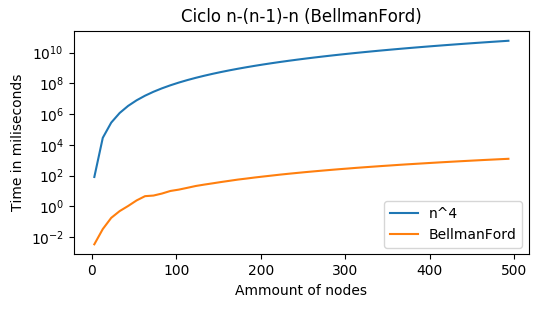
\includegraphics[height = 4.5cm,width = 9cm]{BFlog-nnl1n.png}
\end{figure}
\pagebreak

Y lo que podemos notar hasta ahora es que la cota propuesta es muy grosera. Entonces, si observamos los siguientes graficos correspondientes a la instancia Todos unos:

\begin{figure}[h]
    \caption{El primer gr\'afico (izquierda) corresponde a el tiempo de ejecuci\'on dividido por la complejidad te\'orica.}
    \caption{El segundo corresponde a las comparaciones en escala logar\'itmica.}
    %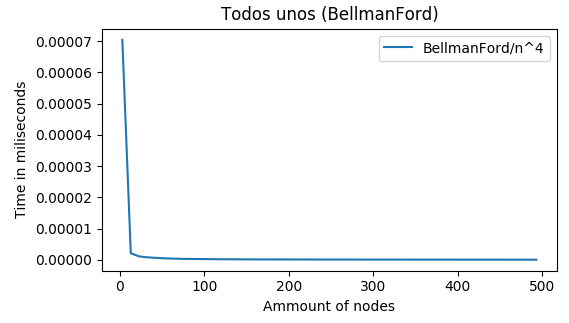
\includegraphics[height = 6cm,width = 9cm]{B-F4unos.png}
    %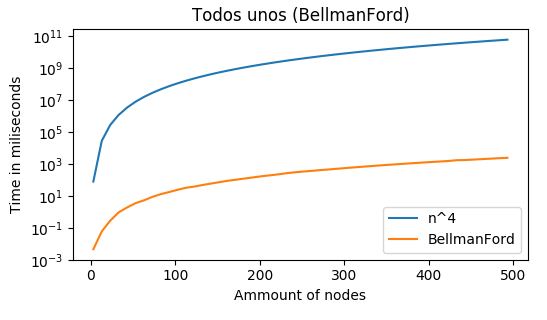
\includegraphics[height = 6cm,width = 9cm]{BFlog-unos.png}
    	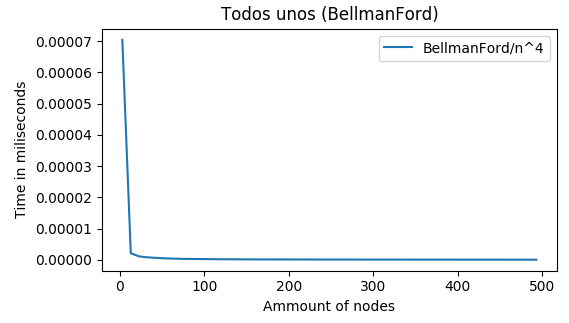
\includegraphics[scale=0.6]{B-F4unos.png}
    	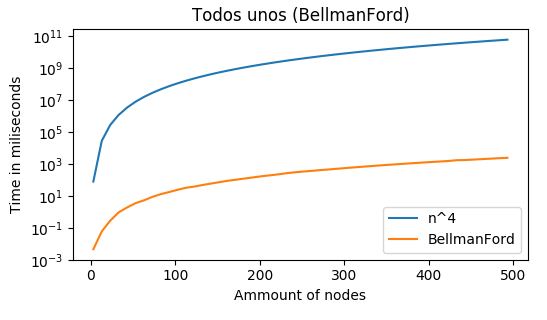
\includegraphics[scale=0.6]{BFlog-unos.png}
\end{figure}

Podremos llegar a dos an\'alisis: como mencionamos antes, la cota ser\'a muy grosera y esto se puede notar en los dos gr\'aficos pero m\'as que nada en el primero, ya que de dividir nuestro tiempo de ejecuci\'on actual por la complejidad propuesta resulta una funci\'on que tiende a cero asint\'oticamente, lo cual nos indica que efectivamente $\mathcal{O}$($n^{4}$) ser\'a una cota superior.

Y lo segundo que podemos mencionar es que a diferencia de lo afirmado previamente, el caso en el que todas las divisas tienen tasa de cambio 1 entre s\'i, es peor que el caso Ciclo $d_{n}-d_{n-1}-d_{n}$.

En cuanto a lo primero, si vemos los siguientes gr\'aficos en los cuales dividimos el tiempo de ejecuci\'on del caso Todos unos por $n^{3}$ y $n^{2}$ respectivamente:

\begin{figure}[h]
%	\begin{center}
%		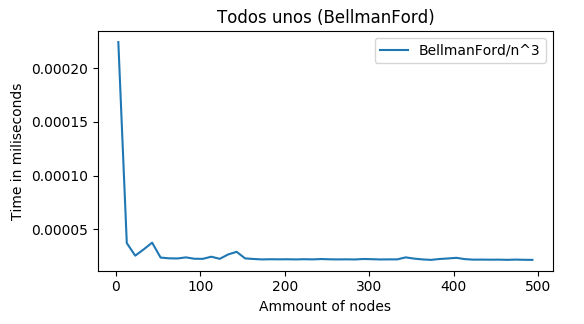
\includegraphics[height = 6cm,width = 9cm]{BF3-unos.png}
%    	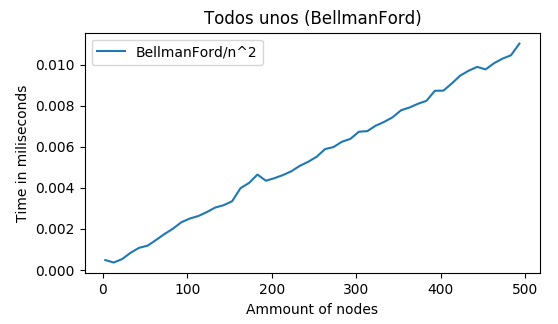
\includegraphics[height = 6cm,width = 9cm]{BF2-unos.png}
%	\end{center}
		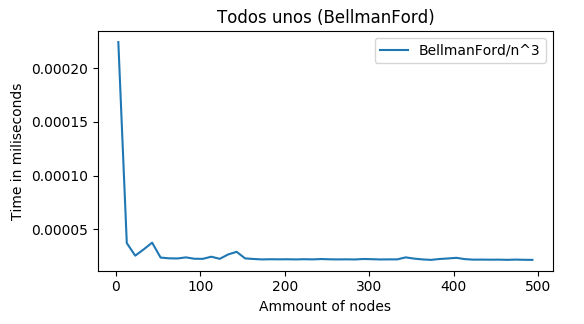
\includegraphics[height = 6cm,width = 9cm]{BF3-unos.png}
    	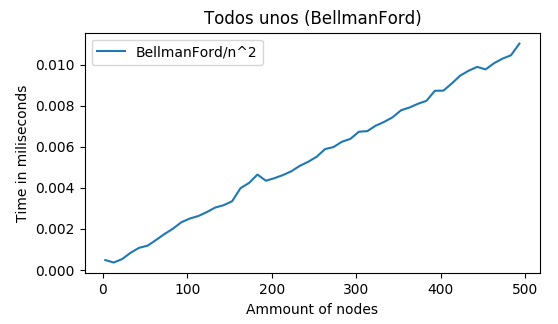
\includegraphics[height = 6cm,width = 9cm]{BF2-unos.png}
\end{figure}

Podremos ver que reci\'en cuando dividimos por $n^{2}$ tendr\'emos una funci\'on lineal que inclusive tendr\'a una pendiente muy chica lo cual confirmar\'ia que $\mathcal{O}$($n^{4}$) es una cota muy grosera pero que sigue sirviendo como cota superior.
Por lo tanto podemos concluir: nuestro algoritmo cumple que en la pr\'actica, su complejidad te\'orica es una cota superior.
\\
\begin{center}
  \rule{100mm}{0.1mm}  
\end{center}


Ahora, formularemos la hip\'otesis correspondiente a nuestra segunda aproximaci\'on:

\begin{itemize}
    \item[•] \textbf{Hip\'otesis FW:} El algoritmo que resuelve el problema de arbitraje que usa la idea del algoritmo de Floyd-Warshall como intermedia tendr\'a una complejidad pr\'actica a lo sumo igual que la de su complejidad te\'orica: $\mathcal{O}$($n^{3}$), y la complejidad pr\'actica de todos los casos (peor, mejor, promedio) ser\'a muy parecida.
\end{itemize}

Observaci\'on: Para este algoritmo usaremos todas las instancias previamente mencionadas.

Entonces, empezando con los gr\'aficos con escala logar\'itmica:


\begin{figure}[h]
    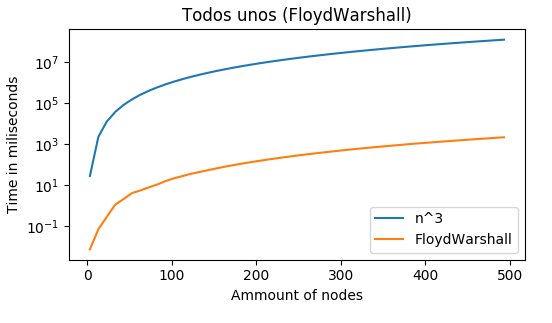
\includegraphics[width=0.55\textwidth]{FWlog-unos.png}
    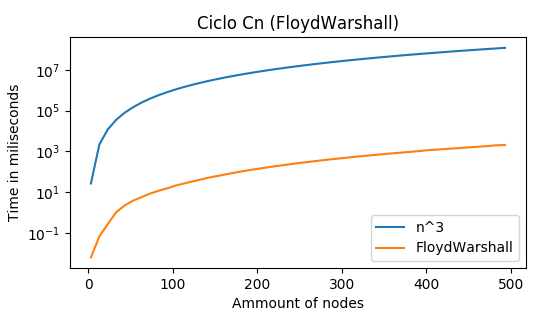
\includegraphics[width=0.55\textwidth]{FWlog-cn.png}
    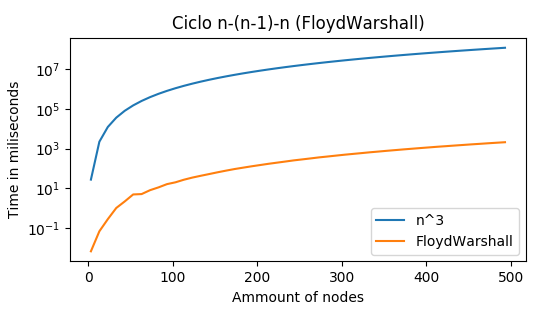
\includegraphics[width=0.55\textwidth]{FWlog-nnl1n.png}
\end{figure}

Si observamos todos estos gr\'aficos podemos observar que distintos casos de ejecuci\'on del mismo algoritmo las cuales, algunas tienen soluci\'on (Ciclo $d_{n}-d_{n-1}-d_{n}$ y Ciclo $C_{n}$) y otras no (Todos unos) tendr\'an curvas muy similares, lo cual validar\'ia la segunda parte de nuestra hip\'otesis. 

Adem\'as podemos notar que aqu\'i tambi\'en la complejidad te\'orica ser\'a una cota. Para poder ver esto mejor veremos los siguientes gr\'aficos:

 \begin{figure}[h]
     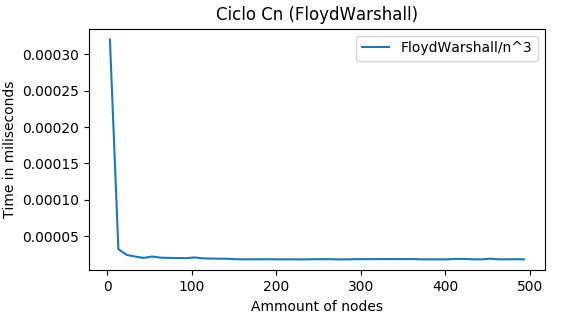
\includegraphics[height = 5cm,width = 9cm]{F-W3cn.png}
     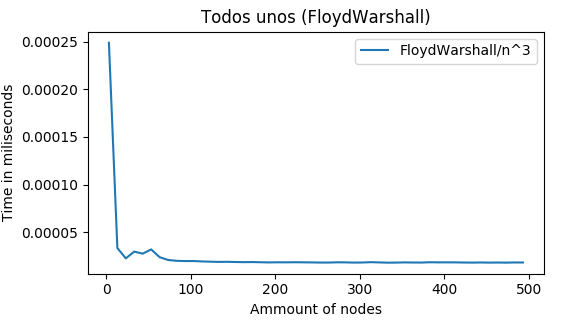
\includegraphics[height = 5cm,width = 9cm]{F-W3unos.png}
     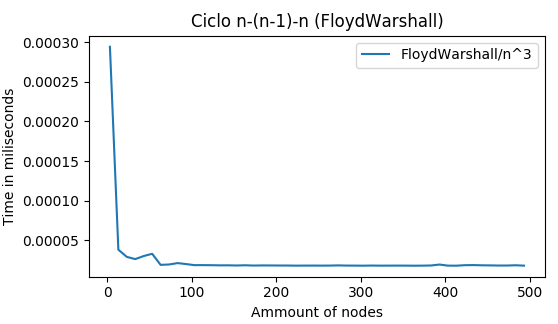
\includegraphics[height = 5cm,width = 9cm]{FW3-nnl1n.png}
 \end{figure}
 \pagebreak
 
 De lo que podremos concluir: al igual que con nuestro anterior experimento, la complejidad te\'orica ser\'a una cota superior grosera, y esto har\'a que al dividir nuestro tiempo de ejecuci\'on por la misma resulte una funci\'on que tiende a cero. Es decir, $n^{3}$ tender\'a a infinito m\'as r\'apido en tiempo de ejecuci\'on que nuestra funci\'on propuesta, lo cual nos permite asegurar que la complejidad te\'orica ser\'a una buena cota superior.

%Esto puede no ir quiza, hay que verlo
%\section{Comparaciones de algoritmos de los problemas resueltos}

\pagebreak
%AGREGAR PAPER DE C.T. ZAHN !!!!!!!!!!!!!!!
\section{Bibliografía}
\begin{itemize}
	\item \url{https://en.wikipedia.org/wiki/Cluster_analysis}
	\item \url{https://en.wikipedia.org/wiki/Principles_of_grouping}
	\item \url{https://towardsdatascience.com/unsupervised-learning-and-data-clustering-eeecb78b422a}
	\item \url{https://towardsdatascience.com/supervised-vs-unsupervised-learning-14f68e32ea8d}
	\item \url{https://machinelearningmastery.com/supervised-and-unsupervised-machine-learning-algorithms/}
\end{itemize}

\end{document}
